% !TeX document-id = {e267d368-ee0e-4347-96b8-d2202efb2395}
% !BIB TS-program = biber
% !TeX encoding = UTF-8
% !TeX spellcheck = en_GB
\documentclass[12pt, a4paper]{extarticle}

%\usepackage{showframe}

\usepackage{cmap}					% поиск в PDF
%\usepackage{mathtext} 				% русские буквы в формулах
%\usepackage[T2A]{fontenc}			% кодировка
\usepackage[utf8]{inputenc}			% кодировка исходного текста
\usepackage[english]{babel}			% локализация и переносы
%\usepackage[urw-garamond]{mathdesign}
%\usepackage{indentfirst}
\usepackage{setspace}
\frenchspacing % добаляет большой пробел между предложениями
%\onehalfspacing
\linespread{1.5}
%\usepackage{helvet}
%\usepackage{newcent}
%\usepackage{lmodern}
\usepackage{calligra}
\DeclareFontFamily{OT1}{pzc}{}
\DeclareFontShape{OT1}{pzc}{m}{it}{<-> s * [1.10] pzcmi7t}{}
\DeclareMathAlphabet{\mathpzc}{OT1}{pzc}{m}{it}

\DeclareUnicodeCharacter{0301}{} %workaround

\usepackage{gensymb}
\usepackage{textcomp}
\usepackage{booktabs}
\usepackage{makecell}
\usepackage{pdflscape}
\usepackage{tabularx}
\usepackage{graphicx}
\usepackage{rotating}

%БЛОК СООТВЕТСТВИЯ ПРАВИЛАМ
%\renewcommand{\rmdefault}{ftm}
\usepackage{times}

%without babel
\renewcommand{\contentsname}{CONTENTS}
\renewcommand{\refname}{REFERENCES}

\makeatletter
% запрещаем переносы в названиях секций
%\renewcommand{\section}{\@startsection{section}{1}{0pt}%
%	{-3.5ex plus -1ex minus -.2ex}%
%	{2.3ex plus .2ex}%
%	{\centering\hyphenpenalty=10000\normalfont\bfseries}}

% chapter
\usepackage{titlesec}
\titleformat{\chapter}{\thispagestyle{myheadings}\centering\hyphenpenalty=10000\normalfont\huge\bfseries}{
	\thechapter. }{0pt}{\large}
\makeatother

%section
%\titleformat{\section}[block]{\bfseries\large\filcenter}{SECTION \thesection.}{.5em}{}
\titleformat{\section}[block]{\bfseries\filcenter}{}{.5em}{}

% subsection
\titleformat{\subsection}[block]{\bfseries\filcenter}{\thesubsection.}{.5em}{}

%subsubsection
\titleformat{\subsubsection}[block]{\bfseries\filcenter}{\thesubsubsection.}{.5em}{}

%math font size (textfont-disp-script-scriptscript)
\makeatletter
\DeclareMathSizes{\f@size}{12}{10}{9}
\makeatother

%to show current font size in log (14pt = 14.4pt)
\makeatletter
\show\f@size
\makeatother

%toc depth
\setcounter{tocdepth}{2}

%TOC section cap
%\addto\captionsenglish{
%	\renewcommand{\contentsname}{\hfill\bfseriesCONTENTS\hfill} 
%}
%\makeatletter
%\renewcommand{\tableofcontents}{%
%	\vspace*{-4mm}% reduce space before
%    \noindent{\contentsname}%
%	\vspace{2mm}% space between title and rule
%	\hrule
%	\vspace{2mm}% space below rule
%	\@starttoc{toc}}
%\makeatother

%bib section cap
%\DefineBibliographyStrings{english}{%
%	bibliography = {BIBLIOGRAPHY},
%	references = {REFERENCES},
%}


% КОНЕЦ БЛОКА СООТВЕТСТВИЯ ПРАВИЛАМ



%bibstyle=gost-authoryear-min,
%citestyle=authoryear,
%работа с библиографией
%style=authoryear
%sorting=nyt,
\usepackage[style=apa,
			maxcitenames=1,
			%maxnames=10,
			backend=biber]{biblatex}
\addbibresource{../Sources/lit.bib}

%Убрать тире из библиографического списка
%\renewcommand*{\newblockpunct}{\addperiod\space\bibsentence}.:
%Для возврата к прежнему значению (установленному по умолчанию):
%\renewcommand*{\newblockpunct}{\addperiod\addnbspace\textemdash\space\bibsentence}.



%Дополнительные пакеты
\usepackage{amsmath,amsfonts,amssymb,amsthm,mathtools} %математика
\usepackage{indentfirst} %отступ первого абзаца
\usepackage{graphicx} %вставка рисунков
\usepackage{wrapfig} %обтекание рисунков текстом
\usepackage{geometry} %установка полей
\geometry{top=20mm} % >20
\geometry{bottom=30mm} % >20
\geometry{left=35mm} % =35
\geometry{right=20mm} % >15
\usepackage{soul} %модификаторы начертания
\usepackage{csquotes}
%\usepackage{titling}
\usepackage{enumitem}
\usepackage[toc,page]{appendix}
\usepackage{tocloft}
\usepackage{siunitx}
\usepackage{multicol}

\renewcommand{\appendixtocname}{Annex}
\renewcommand{\appendixname}{Annex}
\renewcommand{\appendixpagename}{Annex}
\renewcommand{\cftsecleader}{\cftdotfill{\cftdotsep}}

\makeatletter
\newcommand{\mathleft}{\@fleqntrue\@mathmargin0pt}
\newcommand{\mathcenter}{\@fleqnfalse}
\makeatother

\usepackage{float}
\usepackage{hyperref}
\usepackage[usenames,dvipsnames,svgnames,table,rgb]{xcolor}
\hypersetup{				% Гиперссылки
	unicode=true,           % русские буквы в раздела PDF
	pdftitle={Determining Exchange Rate Pass-through in Russia},   % Заголовок
	pdfauthor={Artur N. Zmanovskii},      % Автор
	pdfsubject={Macroeconomerics, Macroeconomics},      % Тема
	pdfcreator={}, % Создатель
	pdfproducer={}, % Производитель
	pdfkeywords={Pass-through} {ERPT} {PERR}, % Ключевые слова
	colorlinks=true,       	% false: ссылки в рамках; true: цветные ссылки
	linkcolor=black,          % внутренние ссылки
	citecolor=black,        % на библиографию
	filecolor=black,      % на файлы
	urlcolor=black           % на URL
}

\makeatletter
\def\blfootnote{\gdef\@thefnmark{}\@footnotetext}
\makeatother

%колонтитулы
\usepackage{fancyhdr} %загрузим пакет
\pagestyle{fancyplain} %применим колонтитул
\fancyhead{} %очистим header на всякий случай
%\fancyhead[LE,RO]{\thepage} %номер страницы слева сверху на четных и справа на нечетных
%\fancyhead[CO]{текст-центр-нечетные}
%\fancyhead[LO]{текст-слева-нечетные} 
%\fancyhead[CE]{текст-центр-четные} 
\fancyfoot{}
%\fancyfoot[RE,RO]{\thepage}
\rfoot{\thepage}
\renewcommand{\headrulewidth}{0pt}
\setcounter{page}{2}

%шапка
\title{{\large DETERMINING EXCHANGE RATE PASS-THROUGH IN RUSSIA}}
\author{Artur N. Zmanovskii\footnote{National Research University `Higher School of Economics'}}
\date{}

%\renewcommand{\appendixname}{Appendix}

\begin{document}
\setcounter{page}{2}
\begin{abstract}
	Russian inflation movements are mostly associated with exchange rate fluctuations, especially after decision of Bank of Russia to adopt floating exchange rate regime. Several studies attempt to measure exchange rate pass-through for Russia, although their estimations are shock-independent. This work estimates SVAR and applies sign and zero restrictions in order to recover shock-dependent ERPT to describe effects of exchange rate to prices under different structural shocks. My findings are comparable to ones in the literature and show that oil shock pass-through in both short- and long-run is ambiguous: while the effect to CPI is low, it is huge to core CPI.
\end{abstract}
\newpage

\tableofcontents
%\maketitle
\linespread{1.5}

\newpage
%\tableofcontents
%\newpage
\linespread{1.5}

\section*{SECTION 1. INTRODUCTION}
\addcontentsline{toc}{section}{SECTION 1. INTRODUCTION}

\blfootnote{\textit{To the memory of my grandfather. Bene qui latuit, bene vixit.}}
The process of integrated world economy formation has been quite substantially changing policies of monetary and macroprudential authorities around the world, adding more challenges to them. Emerging economies being involved into world market has been experiencing a huge policy transformation, especially for ex-socialist countries with strict authoritarian regimes that had very basic international trading affairs before the collapse of these regimes. During transitory process of integration into world economy for such countries, it appears that price stability there becomes subject not only to domestic shocks, but shocks coming from outer world.

The main goal of a monetary authority is price stability; in the above mentioned conditions, policymakers of emerging economies are not suited well for rebuffing outer shocks, since the natural mechanisms of self-compensation in the local economy are yet to be founded. This fact requires prudent policy adjustment, which takes into account a structure of international trade, exchange rate fluctuations and external shocks occurring globally. 

To render the basis for this, the policymaker has to conduct not only positive, but normative analysis of the economy and find transmission channels of external shocks into inflation to guarantee price stability. As there is external trade, one should be interested in effect of exchange rate fluctuations to domestic prices, usually observed in the literature as exchange rate pass-through.

Russia, as emerging ex-socialist commodity economy, can be described as severely subject to commodity (oil) shocks and exchange rate fluctuations. During last 30 years, ruble --- local currency of Russia --- has experienced several large depreciation waves (the largest ones were after 1998 default and 2014 oil price drop). Accompanied by different set of shocks, these events had different degree of exchange rate pass-through in the Russian economy. 

There is many research done on shock \textit{independent} pass-through estimation made for many countries; several papers estimate it for Russia, some of them getting though controversial results due to lack of data available. This approach, in a plain setup, does not require sophisticated statistical methods, as estimates can be obtained from OLS model.

On the other hand, more methods have been developed for the purpose of estimation of shock-dependent exchange rate pass-through for the last 10 years. These methods appear to be applied for developed economies (Euro area, US), while, at the moment of writing this work and my personal knowledge, there is only one work estimating shock-dependent pass-through for Russia based on inference from DSGE (\cite{Khotulev2020}). Disappointingly, there are no works for Russia that employ structural vector autoregressions, which are more data-driven and widespread in the literature.

The purpose of this work is to estimate shock-dependent exchange rate pass-through for Russian economy using structural vector autoregression, closing a gap in the literature. I include five variables from 2003Q2 to 2020Q4 into two models, depending on CPI composition: oil price, short-term interest rate for Russia, ruble nominal effective exchange rate, Russian real GDP and CPI (full or core) in order to calculate price-to-exchange rate ratio for five structural shocks: global persistent shock, local monetary shock, local exogenous exchange rate shock, local supply shock and local demand shock. I use quarterly data in order to estimate the model since there is no monthly time series for Russian output.

In order to identify structural shocks, after estimation of vector autoregression, I apply short-run sign and zero restrictions proposed in (\cite{Arias2014}). Although signs of impulse response functions need to be guessed, this method is quite flexible and allows to precisely estimate shock-dependent exchange rate pass-through. To address problem of weak identification, I estimate Bayesian VAR with uninformative Normal Inverse-Wishart prior and use identification scheme mentioned above for 500 draws from posterior distribution. 

In general, my findings meet results from (\cite{Khotulev2020}) for monetary and global persistent (oil) shocks. Pass-through estimate from purely exogenous exchange rate shock is comparable to shock-independent ones captured in the literature about Russia and CIS. Analysis reveals highest pass-through estimate from exchange rate shocks, while oil fluctuations, which are commonly considered as a main driver of exchange rate for Russia, have a little pass-through effect. However, pass-through is higher in Russia comparing to developed economies (US and Euro area), which is expected.

Another result that may be interesting for a reader is historical decomposition of Russian CPI growth rate (both full and core), which shows contribution of different macrovariables in the model to inflation volatility. There is a presence of price puzzle after 2014 rouble depreciation, although monetary shocks to core CPI from the beginning of 2020 and to full CPI in the last quarter of the same year become positive. Talking about COVID-19 outbreak in the first quarter of 2020, I conclude that the main drivers here were global persistent (associated with oil price) and local supply shocks, while exchange rate was cooling down consumer inflation. In the last quarter of 2020 gradual increase in oil price reduced inflation rate, while exchange rate effect appears to be positive; I associate the latter with a political incident in late summer of the same year.

This paper is organised as follows. Section 2 guides reader through the literature on the topic of exchange rate pass-through. For convenience, I break this section into two parts: a) methods and non-CIS economies and b) Russia and CIS countries. Section 3 gives a brief econometric introduction and defines the model and identification schemes used. Section 4 describes data used in this work. Section 5 reveals results fetched from the model. Section 6 concludes.

\newpage
\section*{SECTION 2. LITERATURE REVIEW}
\setcounter{section}{2}
\addcontentsline{toc}{section}{SECTION 2. DATA}
The goal of pioneering works in exchange rate pass through estimation area was mainly in determining industry-specific effects in specific economies: among others, (\cite{Schembri1985}) examines Canadian exports, (\cite{Menon1992, Menon1993}) --- Australian exports and Imports of Motor Vehicles, (\cite{Khosla1991, Athukorala1994}) --- Japanese exports, (\cite{Cowling1989} --- UK and West German car market, \cite{Athukorala1991} --- Korean exports, \cite{Baldwin1988, Feenstra1989, Hooper1989}) --- US imports. These papers show that there is a heterogeneity in pass-through across industries as well as countries though challenging data measurement errors and model misspecifications. A huge contribution to review these attempts is made in (\cite{Menon1993, Menon1995}).

Looking for exchange rate pass-through for whole economies, \autocite{Khosla1989} estimate shock-independent ERPT to export prices for 23 countries using calculated quarterly nominal effective exchange rate for each economy and fitting OLS regressions. They find that pass-through effect varies drastically across countries: for developed economies this value is high, meanwhile developing ones experience low pass-through.

A more advanced methods are used in (\cite{Kim1990}) --- author examines pass-through to US import prices and influence of exchange rate to mark-up using a model with time-varying parameters. It is shown that a mark-up negatively correlates with US dollar exchange rate, though a direct effect of the latter to prices fell from 1980s. 

In (\cite{Deravi1995}) a vector autoregression (VAR) is applied to fit US broad money aggregate, dollar exchange rate and consumer price index (CPI) with a main emphasis on monetary supply shock. Via causality test It is underlined that there is a significant causality effect of broad money to other macrovariables. Variance analysis suggests the effects to CPI from innovations to other two variables are nearly equal after four years.
 
(\cite{Kim1998}) employs vector error-correction model (VECM) in order to study pass-through to US import prices. This paper reveals a significant negative effect of US exchange rate appreciation to producer price index (PPI) and conducts causality test for this dependency, which confirms an influence of exchange rate. Moreover, author argues that previous works were using inefficient methods to examine ERPT. 

%Taylor2000
In his renown paper, \textcite{Taylor2000} provides strong theoretical framework for understanding exchange rate pass-through nature. The author simulates three-equation model of individual and aggregate prices and output and shows that when the inflation is low, pricing power of firms declines as well leading to lower pass-through. Hence, if a producer wants to raise or lower their individual price due to change in costs or, equivalently, exchange rate, he or she would expect other firms stay on the remaining price level due to low inflation.
 
%DSGE-like papers
Another approach of examining exchange rate pass-through is contained in literature based on general equilibrium models, although there are few ones specially structured for studies in this particular field. Mainly based on purely statistical approach, this particular paper refers only to several works of this kind, leaving the rest to the reader.

One of the works is \cite{Adolfson2001}, where author examines optimal policy of monetary authority under different completeness of pass-through. The main consequence of this study is that the lower pass-through is, the less important nominal economy is, as interest rate response to shocks from outside is lower and exchange rate fluctuations are higher.

The seminal paper in this field is \cite{Obstfeld2002}. It does not directly touch the pass-through problem, however, it is a starting point for many papers in this field. In the paper, a cooperation of monetary authorities in a two-country model is examined. The main result of this paper is that even if monetary authorities do not coordinate with each other, benefits from macroeconomic stabilization can outweigh lack of coordination, and coordination under fixed exchange rate is more preferred than one under the floating rate.

Looking for effects of exchange rate volatility, (\cite{Devereux2002}) develop a multi-economy new-Keynesian general equilibrium model based on the model from aforementioned paper. Authors show that fluctuations in nominal exchange rate appear to compensate pass-through to prices nominated in local currencies. It is argued that even if there is a little volatility in fundamental macroeconomic variables, fluctuations of exchange rate may be quite high. This model lacks empirical research though, constrained only by simulations with different parametrisation.

Basing on the same foundations, an attempt to make an empirical research based on DSGE model is done in (\cite{Smets2002}), where Euro area data is used to calibrate a model and estimate exchange rate pass-through in an economy with optimal monetary policy. As a result, authors claim that under an assumption of presence of import price stickiness in the economy, its effect is similar as stickiness of domestic prices.

%Pretty not DSGE
\textcite{Gagnon2004} use Monte-Carlo approach with multi-equation model to show that there was a decline in exchange rate pass-through since 80s due to inflation stabilisation policy conducted by many central banks across the world. To find more evidence, authors fit an OLS regression with lags of exchange rate summed with foreign CPI for two subsamples individually chosen for 20 countries. Additionally, they estimate interest rate rule coefficients in order to find changes in monetary policy. Finally, authors argue that the hypothesis is confirmed.

%Current Empirics
A new wave in studying exchange rate pass-through --- use of structural vector autoregressions (SVAR) --- starts from (\cite{Hahn2003}) for Euro area macro data from 1971 to 2002. In this remarkable work, a recursive (also known as \textit{Cholesky}) identification scheme is used in order to recover macroeconomic shocks to PPI and HICP from other different macroeconomic variables (oil price, interest rate, output gap and non-oil import prices). To address statement about pass-through decline in (\cite{Gagnon2004}), author conducts a robustness test and finds out that there was no significant change in pass-through effect for the Euro area.

The same conclusion about decline, among other ones, is made in (\cite{Campa2005}). Searching for the pass-through effect to import prices, authors examine data for 23 countries and assert that the pass-through effect is incomplete for all countries in the short run and for overwhelming majority of them in the long run.

(\cite{CaZorzi2007}) and (\cite{McCarthy2007}) papers resemble previously cited (\cite{Hahn2003}). The first work studies data for 12 developing economies and employs recursive SVAR to estimate shock-dependent ERPT; authors find that pass-through effect fades down to the distribution chain and argue that when inflation in a developing economy is low, ERPT is comparable to one of developed countries.

On the opposite side is (\cite{McCarthy2007}) work, where data for nine developed countries are examined applying Cholesky identification scheme to VAR. Author states that pass-through in developed economies is quite low, and inflation in the US is mainly driven by oil shocks, producer price shocks and internal CPI shocks.

In (\cite{Shambaugh2008}) paper author uses long run restrictions for SVAR in order to identify link between exchange rate and CPI together with import prices. Author uses data for 16 countries for the time frame from 1973 to 1999 and obtains supportive evidence that low inflation declines pass-through --- for some countries, CPI growth rate does not respond to exchange rate shocks in the same magnitude as producer price index growth rate.

Data's granularity higher than quarterly is not usually found in the studies, although (\cite{Amstad2010}) observe monthly Swiss CPI and NEER from 1993 to 2008. This work employs event study approach to estimate an effect of monthly import price time series release to ERPT. Author underlines that this method is more suitable for policymakers due to possibility of using the most current data and does not rely on VAR restrictions, which may be controversial. The criticism of SVAR is quite questionable in this light, since the monthly data does not impair a possibility of proper identification of shocks, while the benefits of shock-dependent ERPT are higher for monetary and macroprudential authorities.

An innovative identification method is introduced by \textcite{An2012} --- author employs sign identification scheme in order to obtain price-to-exchange rate ratio (\textit{PERR}, shock-dependent exchange rate pass-through), which will be described in the following Section. Author fits the model for eight developed economies and claims that for the most cases pass-through is incomplete. Another conclusion is that pass-through is higher for small-sized economies with more volatile monetary policy.

The work of \textcite{Delatte2012} is devoted to determination of pass-through asymmetry for four countries (Germany, Japan, UK, US) from 1980 to 2009. An ARDL with nominal exchange rate changes divided into two variables (with positive and negative increments) is estimated to determine both short-run and long-run asymmetric ERPT. Author argues that pass-through is smaller during local currency appreciations.

(\cite{BrunAguerre2012}) paper's aim is to find what drives ERPT to import prices. Authors use both ECM and panel fixed effects (FE) model to catch time- and country-specific effects for 37 countries on 1980--2009 period; again, pass-through asymmetry is considered. The conclusion is that there is no evidence of pass-through declining for both developed and emerging economies, although domestic tariffs and import-to-export ratio matter.

Monthly data of Taiwanese economy under deflation are examined in (\cite{Lin2012}). In this work, a two- and three-regime threshold autoregression (TAR) models are fit to find non-linearities in pass-through relation. It is argued that pass-through declines only when inflation is close to zero, and the link of ERPT and inflation is V-shaped. With this non-trivial result, high rates of deflation are unpleasant for an economy additionally from the side of exchange rate pass-through.

Another work observing Asian economy is (\cite{Jiang2013}). Authors estimate SVARs with custom shock matrix in order to find PERR for China. This method is more flexible than recursive identification scheme as the shock matrix does not necessarily need to be triangular, although application of such scheme is quite situational. Authors conclude that PERRs are incomplete, which is usual for the literature in this field.

(\cite{Yamada2013}) paper is devoted to study exchange rate regime effect to inflation among developing and emerging economies. Author fit treatment effects model with propensity score matching based on GDP and geographical characteristics in order to calculate between inflation targeting regime and other ones. The conclusion is that inflation targeting exchange rate regime performs at least not worse than fixed regime in terms of inflation lowering.

Multi-currency study for 17 countries of Euro area is done by \textcite{Bandt2014} to estimate effect of exchange rate fluctuations to import prices for multiple trade partners. Currencies chosen are US dollar, UK pound-sterling and Chinese Renminbi. Authors estimate FE model in order to calculate ERPT and find out that in the short run pass-through is incomplete, but its completeness is confirmed fore the long run.

In order to look for the changes in pass-through after 2008 financial crisis, \textcite{Jasova2016} estimate 6-year rolling ERPT for both developing (11) and advanced (22 countries) economies completing their study by fitting two-way FE model. Authors assert that pass-through declined during financial crisis for developing economies, meanwhile ERPT of developed countries remained on a relatively stable level.

In (\cite{Comunale2017}) paper data for four Euro area countries --- France, Germany, Italy and Spain --- are studied to find both ERPT and PERR under the zero lower bound (ZLB) environment. Instead of short-term interest rate, authors make use of calculated \textit{shadow interest rates} and estimate Bayesian VAR with sign and zero restrictions. The results of the study are that pass-through is high and volatile to import prices and, in general, is dependent on shocks evolving. Moreover, authors state that the process of choosing identification scheme is quite sophisticated, and the identified shocks are true only conditional on the scheme involved.

Both FE model and sign and zero restricted SVAR are estimated in (\cite{Forbes2017}), where authors try to analyse time- and country-specific differences in pass-through on the sample of 26 countries. It is argued that structural variables, like the first two statistical moments of inflation and exchange rate are important for time and country effect explanation, while structural shocks are crucial for explanation of macro-variable variation in time.

A quite remarkable paper of the same collective is (\cite{Forbes2018}). Authors study UK economy pass-through before and during Brexit using SVAR model with sign and zero restrictions. The study shows that pound-sterling's depreciation periods during 2008 financial crisis and Brexit have different ground and discrepancy in inflation rates are caused by different shocks affecting the economy. Authors admit that set up in this fashion, a model cannot capture all the complexity of pass-through nature, although identification of shocks can help to improve relevant policy by monetary authority.

Another work employing the same method is (\cite{An2020}), though \textit{narrative} sign restrictions (simply put, signs dictated by historical events) are added. The main drivers of Japanese pass-through are examined in this study. Authors argue that narrative sign approach is more promising in terms of shock identification procedure.

Time-varying ERPT is examined in (\cite{LeivaLeon2019}), where authors estimate time-varying parameters (TVP) dynamic factor model and SVAR with sign restrictions for Euro area. A TVP approach is quite innovative in pass-through literature, as it is highly likely to solve problems of non-linear ERPT estimation. The paper's conclusion is that inflation is mostly driven by exogenous exchange rate shocks, though core inflation are less exposed to these fluctuations.

\textcite{Colavecchio2019} use local projection method in order to capture non-linear pass-through effects for the 19 countries in Euro area. Plainly speaking, local projections are \textit{h}-ahead forecasts on the basis of current data. The results show that there is no complete pass-through for all the countries neither after a one year nor two years. Authors also find there is a sign and exchange rate shock size non-linearity for some countries.

The recent work of \textcite{Comunale2020} is devoted to a comparison of Bayesian SVARs and DSGEs for the purposes of PERR estimation. This particular work is important in the sense that SVAR and DSGE models can give controversial results; hence, a policymaker needs to distinguish an appropriate aims for both setups. Author finds out that just after a shock PERR's are identical for both models, although in the long-run estimates from DSGE are higher due to endogenous response of macrovariables. 

DSGE is also employed in (\cite{GarciaCicco2020}), where comparison of shock-independent ERPT's and PERR's is done on Chilean data. It is argued throughout the work that pass-through conditional on shocks gives a full picture of macroeconomic variables' relations and that DSGE models are helpful to generate prudent monetary policy. 

In their latest work, \textcite{Forbes2020} estimate both SVAR and FE model for a set of 26 countries in order to review \textit{''shocks vs. structure''} dilemma. Authors claim that both structural characteristics and shocks are important for better understanding pass-through. Also they find an evidence that monetary shocks are associated with large PERR, which made a big contribution to price fluctuations in advanced economies that are not close to the lower bound.

All in all, there has been a shift in the literature from industry-specific studies to understanding of shock importance during exchange rate pass-through estimation. This drift is dictated not only by an evolution of methodology (this point is prevalent though), but data availability and, what is the most important, a switch to macroprudential policy. The intervention of vector autoregressions and Bayesian estimation techniques, especially sign restrictions, have given, in some sense, the second breath to the research. On the other hand, further development of DSGE models and acceptance of them by central banks globally gave an idea of how shock-dependent ERPT should look like for each country. The idea of SVAR being guided by DSGE (at least for a signs) is given in (\cite{Ortega2020}), which is a brilliant review on the topic of exchange rate pass-through estimation with a focus on Euro area and the US.

\begin{center}
	\textbf{Russia and CIS}
\end{center}

One of the first works exploring the Commonwealth of Independent States (CIS) is (\cite{Korhonen2006}), where authors estimate VAR models for each country-member using the data from 1999 to 2004. This work is quite disputable as, for instance, Russia and Kazakhstan have \textit{negative} ERPT, which is highly unlikely even considering the policy in 2000-2005. On the example of Russia, the most obvious omission in this study is that the model is fitted on the data after 1998 default, which led to huge surge in exchange rate due to risk premium shock. After this event, it seems that the ruble was underappreciated, and its exchange rate was lowering from 2000 till 2008 financial crisis together with rise in oil price. Being fitted with this data, VAR may generate biased results, as effects from several shocks are not taken into account: the influence of risk premium shock was declining together with rising oil price shock. Due to this issue, the cited work is a good example why shock-dependent ERPT is important for proper policy implications.

\textcite{Oomes2005} study the relation of inflation and money demand on the example of Russia in 1996--2004. The main focus of this work is economy dollarisation --- the influence of foreign currency holdings in the country. As a side effect, authors estimate ERPT to control for influence of money aggregate to inflation. 

DSGE model for Russia and China is presented in (\cite{Sosunov2006}), where a response of exchange rate to foreign currency accumulation policy by central bank is studied. Analysis shows that low level of money in the economy for Russia in 2001--2005 is a pro-inflammatory factor. Moreover, it is underlined that the management of real exchange rate by means of currency accumulation has a little effect to it.

The model for Russia in \cite{Dobrynskaya2008} is fitted on the sample from 1995 to 2002. This work employs two single-equation regressions (simple and extended ones) in order to estimate ERPT for the country. The choice of time-frame and model (OLS) there is questionable, since the surge of CPI and exchange rate after 1998 crisis probably lead to unreliable estimates, although results in the paper do not contradict economic intuition. Authors argue that exchange rate pass-through in Russia is fast, as a huge part of it comes into inflation right in one month after exchange rate shock.

In (\cite{Kataranova2010}), a more recent (2000--2008) data are used. Author fits different specifications of OLS models accounting for asymmetry in order to evaluate ERPT. The results are that the presence of pass-through asymmetry is confirmed for Russia, and the effect of ruble decline caused by 2008 financial crisis, indeed, was only partial, since the following ruble appreciation strengthen credibility of the local currency.

\textcite{Beckmann2013} estimate exchange rate pass-through for CIS countries on the data from 1999 to 2010. Authors obtain negative ERPT estimate from VAR model for USD-RUB pair and the same estimate close to zero for EUR-RUB pair, which contradicts reality. Authors address this issue by pointing out that this pass-through estimate is shock-independent and there is an uncontrolled effect of oil shocks.

In (\cite{Faryna2016}) paper author estimate bilateral panel VAR for both Russia and Ukraine to study cross-country spillovers. Author claims that depreciation of ruble causes increase in Ukrainian inflation, which follows intuition as Russian and Ukrainian economies have been quite integrated (even after 2014 political crisis this degree of integration remains high). Moreover, it is observed in this paper that inflation in Ukraine responds to USD-RUB changes higher than to USD-UAH (Ukrainian hryvna --- the Ukrainian local currency). 

The other work of the same author is (\cite{Faryna2016a}) examines non-linear ERPT for Ukraine exclusively on the 2007--2016 data. As it is occurred in the literature for Russia, local currency depreciation causes more effect to inflation than its appreciation, although pass-through is higher for Ukraine.

The latest work of \textcite{Faryna2018} studies some CIS countries, including Ukraine and, partially, Russia. This paper employs Global VAR model (VAR with equations for each country) fitted on the 2001--2016 data. This model shows a close relationship of Euro area output and output of CIS countries. An oil shocks is definitely positive for Russia, and what is more interesting, it is positive for CIS countries due to spillover effect.

A VECM model with ERPT asymmetry is used in (\cite{Ponomarev2016}) for 2000--2012 data. Authors break time series into two sub-periods: before and after 2008 financial crisis, to achieve robustness of results. Their findings are that pass-through effect reveals fully in 6-12 month period, and this effect is incomplete.

(\textcite{Comunale2018}) estimate fixed effects panel data model with ERPT asymmetry for CIS countries on a 1999--2014 time-frame. Authors claim that pass-through is high for CIS countries, reaching its maximal level in one year. Moreover, they argue that there is a little evidence of asymmetric pass-through, although it doesn't apply to Russia, as this country is just partially included in the study.

In \cite{Sinyakov2019} authors calibrate a simplified multi-equation static model of small open economy in order to evaluate industry-specific asymmetry of ERPT. Their findings are that electrical appliance manufacturers and paper producers are less likely to transfer costs from exchange rate fluctuations directly to the final good prices keeping ERPT in this area low. On the opposite, textile and wholesale trading industries have very high pass-through (around 0.5--0.6). The final conclusion is that when produces are aware of competitors' actions in a specific industry, the pass-through is high.

A comprehensive research is done by \textcite{Khotulev2020}. In this paper, author evaluate both ERPT by means of OLS model and PERR using the Bank of Russia's DSGE model. There are five exogenous shocks in the latter model: oil price, monetary policy, country risk premium, government expenditures and reserves. A quite disputable result is that there is a huge negative PERR due to government spendings shock (-1.596), which may be a result of purely technical restrictions (first-order approximation of DSGE equations).

The evolution of pass-through literature concerning Russia and CIS is fairly limited, since the last work calculates shock-dependent ERPT. Some works include negative shock-independent ERPT for Russia, which is rather dubious for Russian structure of external trade. Table \ref{table:litreview_erpt} summarizes shock-independent pass-through estimates across the literature.

\begin{table}[h]
	\centering
	\begin{tabular}{llllll}
		Paper                                   & Currency & Data         & Infl. aggr. & Length    & ERPT \\
		\hline
		\cite{Oomes2005}       & NEER               & 1996--2004   & CPI             & Short-run & 0.4--0.5     \\
		\cite{Korhonen2006} & USD & 1999--2004 & ULC\footnote{Unit labour cost.} & Long-run & -0.42 \\
		\cite{Dobrynskaya2008} & NEER               & 1995--2002   & CPI             & Long-run  & 0.35         \\
		\cite{Kataranova2010}  & USD                & 2000--2008   & CPI             & Short-run & 0.06--0.2    \\
		\cite{Beckmann2013}    & USD                & 1999--2010   & CPI             & Long-run  & -0.17        \\
		\cite{Ponomarev2016}   & NEER               & 2000--2012   & CPI             & Short-run & 0.046        \\
		\cite{Faryna2016}      & USD                & 2000--2015   & CPI Core        & Long-run  & 0.1          \\
		\cite{Sinyakov2019}    & NEER               & (2016--2017) & CPI             & Long-run  & 0.35         \\
		\cite{Khotulev2020}    & NEER               & 2005--2019   & CPI             & Long-run  & 0.16        \\
		\hline 
	\end{tabular}
	\caption{Earlier shock-independent ERPT estimates for Russia.}
	\label{table:litreview_erpt}
\end{table}

\clearpage
%%%
\section*{SECTION 3. METHODS}
\setcounter{section}{3}
\addcontentsline{toc}{section}{SECTION 3. METHODS}

\begin{center}
	\textbf{Theoretical Framework}
\end{center}

Before going into technical details, I explain why pass-through estimation is important, and why there may not be complete pass-through (a one-to-one correspondence of exchange rate fluctuations and inflation movements). In this step, I follow (\cite{Comunale2017}) and (\cite{Forbes2018}), which use the most popular approach in the pass-through literature.

First, consider the following aggregate pricing equation of an imported good:
\begin{equation}
	P_t^{imp} = E_t \cdot P_t^{exp, f},
\end{equation}
where $P_t^{imp}$ is price of imported good, $E_t$ is exchange rate and $P_t^{exp}$ is foreign export price. 

Then, taking logarithm on both sides and using $P_t^{exp, f} = Markup_t + MC_t$, we get:
\begin{equation}
	p_t^{imp} = e_t + markup_t + mc_t,
\end{equation}
where $p_t^{imp}$ is a logarithm of import price level, $e_t$ is a logarithm of exchange rate, $markup_t$ is producer mark-up and $mc_t$ is marginal costs. From this relation, any exchange rate fluctuation can be either fully incorporated into import price, or markup and marginal costs can be adjusted. Assuming that firms-exporters are forward-looking, and taking into account price rigidities, one expects mark-up to be adjusted over marginal costs for any macroeconomic shock. 

The same logic, indeed, can be applied to firms-importers, such as electronics and clothing stores for Russia. These firms has marginal costs mainly consisting of foreign wholesale prices of goods imported. Due to price stickiness and oligopolistic nature of the market in these industries, the firms adjust not only the final price of good, nominated in a local currency, but their mark-up. Hence, depending on the shock emerged in the economy, the pass-through can be incomplete.

\begin{center}
	\textbf{Pass-through Definitions}
\end{center}

A simple technique that has been widely used in the literature determining shock-in\-de\-pen\-dent ERPT (\textit{exchange rate pass-through}) is estimation of the following OLS model:
\begin{equation}
	p_t = \beta_0 + \beta^{e}_1 e_t + \beta^{e}_2 e_{t-1} + \beta^{e}_3 e_{t-2} + \beta^{e}_4 e_{t-3} + \ldots+ \varepsilon_t,
\end{equation}
where ellipsis denotes other control variables. Hence, ERPT is calculated as the sum of exchange rate lags coefficients:
\begin{equation}
	ERPT_T = \sum_{j=0}^{T} \beta^e_{t-j},
\end{equation}
where $T$ is an ERPT horizon. An ERPT can be characterised as \textit{incomplete} for a horizon $T$, if $ERPT_T < 1$. 

The most important benefit of this method is its flexibility: a researcher can specify different forms of the price equation, e.g. panel regressions for spatial data, allowing asymmetry of exchange rate effect or time/regime-dependent effects. Non-linear effects are important for studying pass-through dependence on shifts in monetary policy or structural breaks. 

In the same time, ERPT measure lacks identification of economy shocks, which is a huge shortcoming of this approach. This issue is misleading in the sense that it can result into wrong policy conclusions made by authorities: if shock-independent pass-through is measured involving the historical data with a particular set of shocks, the result cannot be applied to the further periods when the economy is exposed to other set of shocks, since ERPT will be different.

In this work I calculate shock-dependent pass-through known in the literature as \textit{price-to-exchange rate} coefficient (PERR). This measure involves estimation of structural vector autoregression, either purely data-driven or derived from DSGE equations. PERR is defined as follows:
\begin{equation}
	PERR^{\text{shock}}_{T} = \frac{\sum_{t=0}^{T}IRF^{\text{shock}, e}_{t}}{\sum_{t=0}^{T}IRF_{t}^{\text{shock}, p}},
\end{equation}
where $IRF^{\text{shock}, \text{response}}_{t}$ is a value of impulse-response function calculated at time $t$ for \textit{response} variable caused by exogenous \textit{shock}. $e$ and $p$ stand for exchange rate and price variables.

\begin{center}
	\textbf{Econometric Model and Identification Strategies}
\end{center}

I estimate two Bayesian vector autoregressions (BVAR) with five variables: oil price in US dollars, local short-term interest rate (MIACR\footnote{Moscow Interbank Average Credit Rate.} 31-180 days), local nominal effective exchange rate, local real GDP index and inflation aggregate (CPI or core CPI). I use two compositions of CPI (full and core) in order to capture pass-through for non-food and non-oil goods, which are mostly imported for Russia. All variables, except interest rate, are used in growth rates in the model.

The choice of variables here is dictated mainly by (\cite{Hahn2003};\cite{Comunale2017}; \cite{Forbes2018}; \cite{LeivaLeon2019}). Throughout the shock-dependent pass-through literature widely used variables are import/export price index, short-term interest rate, exchange rate, output and inflation aggregate. Moreover, the literature uses quarterly data used instead of monthly series due to primarily absence of monthly output data. My work also uses quarterly data, since GDP data estimates are not in free use, while usage of output proxies (e. g. manufacturing index) may lead to controversial results. In addition to this, I include oil price series, as this variable is crucial for determining exchange rate fluctuations and movement of other macrovariables in Russia. More information about data is in the following section.

After VAR estimation a researcher gets its reduced form, which is given as follows:
\begin{equation}
	Y_t = A_1 Y_{t-1}  + A_2 Y_{t-2} + \ldots + u_t,
\end{equation}
where $Y_{t-j}$ is vector of variables' values of lag $j$, $A_i$ is matrix of coefficients at lag $j$, $u_t$ is residual term.

Since variance-covariance matrix $\Xi_{u_t}$ is not diagonal and normalized, there is no economic interpretation of residuals $u_t$. Then, a researcher has to refer to the generalized form of VAR:
\begin{align}
	B_0 Y_t &= B_1 Y_{t-1}  + B_2 Y_{t-2} + \ldots + \epsilon_t,\\
	Y_t &= B_0^{-1}B_1 Y_{t-1}  + B_0^{-1}B_2 Y_{t-2} + \ldots + B_0^{-1} \epsilon_t,\\
	Y_t &= B_0^{-1}B_1 Y_{t-1}  + B_0^{-1}B_2 Y_{t-2} + \ldots + u_t,
\end{align}
From this result and equivalence $B_0^{-1} \epsilon_t = u_t$, an idea is to specify such matrix $B_0$ that a variance-covariance matrix $\Xi_{\epsilon_t} = V(B_0 u_t)$ is diagonal and normalized ($\Xi_{\epsilon_t} = I$). Again, using $B_0^{-1} \epsilon_t = u_t$ a researcher gets:
\begin{equation}
	\Xi_{u_t} = V(B_0^{-1} \epsilon_t) = B_0^{-1} V(\epsilon_t \epsilon_t') B_0^{-1'} = B_0^{-1} I B_0^{-1'} = B_0^{-1} B_0^{-1'}.
\end{equation}
This result is noticeable, as it appears that $B_0^{-1} B_0^{-1'}$ is a Cholesky decomposition of $\Xi_{u_t}$. Then, $\displaystyle\frac{n(n-1)}{2}$ restrictions are needed to exactly identify shocks.

There are several methods to do this. The first method is the simplest one --- naively apply Cholesky decomposition of variance-covariance matrix $\Xi_{u_t}$, in form given above. From this, using as an example choice of variables in this work, shocks are identified as follows:
\begin{equation}
	\begin{pmatrix}
		\epsilon^{\text{Global persistent shock}}_t\\
		%\epsilon^{\text{Global demand shock}}_t\\
		\epsilon^{\text{Mon. shock}}_t\\
		\epsilon^{\text{Ex. rate shock}}_t\\
		\epsilon^{\text{Supply shock}}_t\\
		\epsilon^{\text{Demand shock}}_t\\
	\end{pmatrix} = 
	\begin{pmatrix}
		S_{11} & 0 & 0 & 0 & 0 \\
		S_{21} & S_{22} & 0 & 0 & 0\\
		S_{31} & S_{32} & S_{33} & 0 & 0 \\
		S_{41} & S_{42} & S_{43} & S_{44} & 0 \\
		S_{51} & S_{52} & S_{53} & S_{54} & S_{55} \\
		%S_{61} & S_{62} & S_{63} & S_{64} & S_{65} & S_{66}\\
	\end{pmatrix} 
	\begin{pmatrix}
		u^{\text{Oil}}_t\\
		%u^{\text{Imp. infl}}_t\\
		u^{\text{Int. rate}}_t\\
		u^{\text{NEER}}_t\\
		u^{\text{Real GDP}}_t\\
		u^{\text{CPI}}_t\\
	\end{pmatrix}
\end{equation}
Then, the first variable in the vector is not directly affected by any shock but one that is associated with this variable, while the last variable is affected by fluctuations of all the shocks in the model. The main drawback of this identification scheme is that it implies very stiff restrictions to the shocks, and there may not be desired order of variables that produces sensible result. For example, one can reasonably assume that ruble's exchange rate and inflation have effect to the interest rate in short-run (monetary policy rule reaction).

In the recent literature estimating shock-dependent pass-through, a sign and zero restrictions method is widely used. A reader can refer to (\cite{Arias2014}) for rigorous explanations of this technique, although, in a nutshell, this is a \textit{guess-and-verify} technique: one has to randomly generate matrix $Q$ such that $QQ'$ is diagonal and its product with matrix from Cholesky decomposition produces such IRF's that satisfy both sign and zero restrictions. As the model is underidentified, there are multiple matrices $Q$ satisfying there restrictions. After $n$ times generating the random matrices and obtaining IRF's, their median values are calculated as a result. 

Mostly, this technique is done together with Bayesian estimation of VAR instead of using OLS. This is done mostly for two purposes --- lack of observations and weak identification. Many studies estimate Bayesian VAR with uninformative prior, which adds more flexibility to results. After BVAR estimation, the algorithm proposes to draw several times random estimates and generate big amount of random matrices $Q$. Hence, if identification scheme --- signs and zeros --- are assigned properly, there exist matrices $Q$ for some draws that fulfil these restrictions. 

The main drawback of this approach is that researcher has to intuitively arrange signs of response functions, which is usually non-trivial. (\cite{Ortega2020}) advice to use DSGE models for this purpose, although data are not necessarily to match IRF produced by theoretical justifications.

Taking some ideas from (\cite{An2020}) and basing the sign and zero restrictions mainly on (\cite{Forbes2018}), I use identification scheme described in Table~\ref{tab:signs_and_zeros}. Note that NEER is taken with opposite sign: ruble appreciation yields NEER decrease in my data.

I assume oil price does not respond to any domestic shock, positive supply shock increases GDP and slows down CPI due to excessive supply. Positive demand shock heats up output and inflation, while the central bank fights against it by raising interest rate; foreign importers are required to purchase more local currency, hence, exchange rate declines. \footnote{Though the latter idea may be seem controversial, data comprehensively support it.} Positive exogenous exchange rate shock increases inflation and, as a response, the central bank raises interest rate. Finally, positive global persistent shock is associated with raise of business activity, hence, it pushes up oil price, while oil exporters bring more foreign currency into country, reducing exchange rate.

The model's parsimony is predominantly caused by sign identification issues, while DSGE models may include dozens of variables.\footnote{On the other hand, the process of DSGE model estimation is not the same as the same process for SVAR, as it is either calibration or frequentist/Bayesian estimation of only few parameters.} A lack of identification grows with the number of variables due to requirements of identification schemes and irrelevance of odd variables.

In addition to this, there are no published data for Russian import prices, while almost every study uses them in their analysis. Export prices are also not used, contrary to the literature, as I assume that oil price captures export price shocks, and construction of export price time series would require much effort without necessary data.

\begin{table}[p]
	\centering
	\resizebox{\textwidth}{!}{%
		\begin{tabular}{@{}lccccc@{}}
			\toprule
			Variable & \makecell{Supply shock} & \makecell{Demand shock} & \makecell{Monetary shock} & \makecell{Exchange rate \\shock} & \makecell{Global persistent \\shock} \\
			\midrule
			Real GDP      & +   & +   & -- & ? & ?   \\
			CPI/Core           & -- & +   & -- & + & ?   \\
			Interest rate & ?   & +   & +   & + & ?   \\
			NEER          & ?   & -- & -- & + & -- \\
			Oil price     & 0   & 0   & 0   & 0 & +  \\
			\bottomrule
		\end{tabular}%
	}
	\caption{Identification restrictions used to recover structural shocks. Positive (negative) signs describe non-strictly positive (negative) restrictions for variable's contemporaneous and next quarter response to a particular shock. Zero indicates for no contemporaneous reaction.}
	\label{tab:signs_and_zeros}
\end{table}

\clearpage
\section*{SECTION 4. DATA}
\setcounter{section}{2}
\addcontentsline{toc}{section}{SECTION 4. DATA}

I use quarterly time series of six variables from 2003Q2 to 2020Q4: oil price in USD, short-term interest rate (MIACR 31-180 days), nominal effective exchange rate, real GDP and CPI/Core CPI. Monthly data are available for all the variables, except for GDP, while use of output proxies seems unreasonable as it may distort final results, as inflation-output and exchange rate-output relations are hardly identifiable.

The data time-frame is bounded by the first observation of the real GDP and by its last observation. There are 63 observations in total. CPI is seasonally adjusted according to X13-ARIMA-SEATS; real GDP index is available already seasonally adjusted. NEER is taken with opposite sign, as it is more convenient to work with a direct quote. See Table \ref{table:variables_decription} for data description and sources.

\begin{table}[b!]
	\centering
	%\resizebox{\textwidth}{!}{%
	\begin{tabular}{@{}lll@{}}
		\toprule
		Variable  & Description                                              & Source    \\ \midrule
		Oil price & \makecell[l]{Brent oil price nominated in US dollars, \\quarterly average, QoQ} & Bloomberg \\
		Interest rate & \makecell[l]{MIACR 31--180 days, quarterly average. \\Absent values were imputed by last available rate} & CBR        \\
		Exchange rate & \makecell[l]{Nominal effective exchange rate (NEER) of ruble, \\Ruble appreciation = NEER decline, \\QoQ, Central Bank of Russia methodology} & CBR        \\
		Output        & \makecell[l]{Russian real GDP (2015Q1 = 100), \\seasonally adjusted, QoQ}  & \makecell[l]{FRED} \\
		Inflation & \makecell[l]{Consumer price index and core consumer price index, QoQ, \\seasonally adjusted }          & Rosstat   \\ \bottomrule
	\end{tabular}%
	%}
	\caption{Description of Data and Sources\\	
		CBR = Central Bank of Russia.\\
		FRED = Federal Reserve Economic Data.\\
		OECD = Organization of Economic Co-operation and Development.\\
		Rosstat = Federal State Statistics Service of Russia.\\
		WTO = World Trade Organization.}
	\label{table:variables_decription}
\end{table}

I associate oil price fluctuations with global persistent shock (as in \cite{Forbes2018}), interest rate fluctuations with monetary policy shocks, exchange rate fluctuations with exogenous exchange rate shocks, domestic product fluctuations with supply shocks and CPI fluctuations with demand shocks.
\begin{figure}[b!]
	\centering
	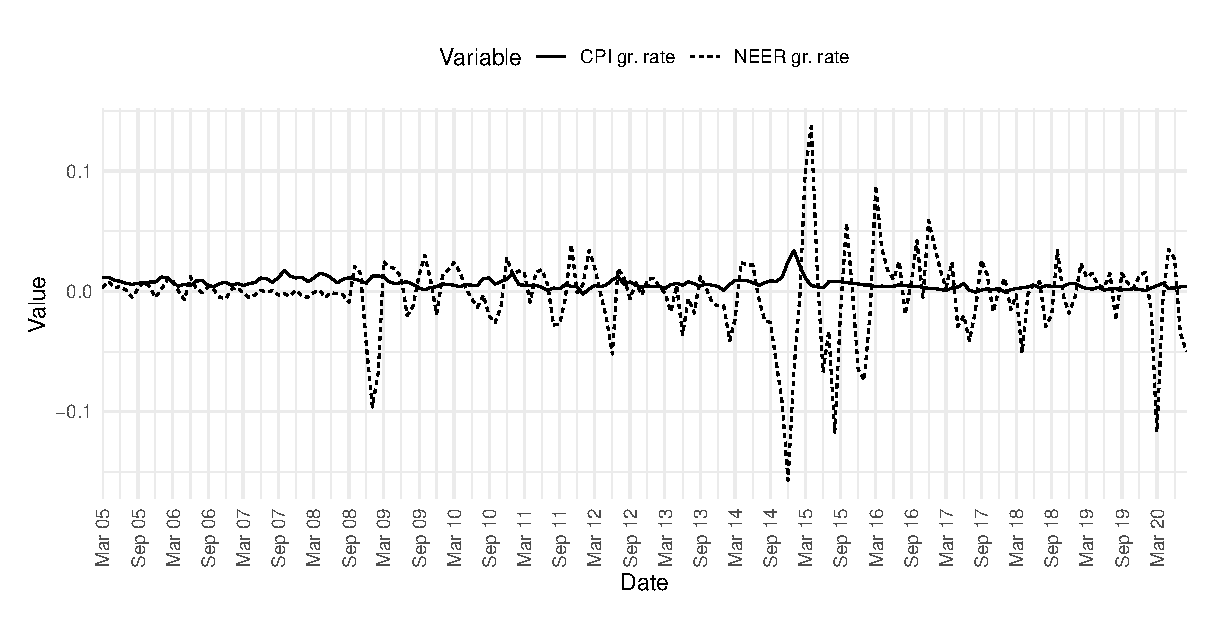
\includegraphics[width=\linewidth]{figures/neer_cpi}
	\caption[]{Time series of NEER and CPI (seasonally adjusted), growth rates.}
	\label{fig:neer_cpi}
\end{figure}

I do not use RUB/USD as the exchange rate, since nominal effective exchange rate is widely used in the literature, and I expect higher values of pass-through coefficients from RUB/USD. Hence, in order to be able to compare results to the literature, I use NEER. 

A quite intuitive fact that oil price is negatively correlated with exchange rate follows from the fact that oil producers convert their yields from convertible currencies (mostly, US dollar and Euro) to Russian ruble, which creates excessive supply of foreign currency. In the same time, ruble appreciation declines consumer prices due to the import-dependent structure of consumer basket (huge share of import in manufactured goods). These relations form a pass-through channel. 

In general, the Russian economy can be described by the following stylized facts:
\begin{enumerate}
	\setlength\itemsep{0.02em}
	\item There is a significant negative correlation of oil price and ruble exchange rate (especially, USD and EUR);
	\item There is a strong negative correlation of interest rate in Russia and Russian GDP;
	\item Oil price and Russian GDP are positively correlated;
	\item Exchange rate and CPI are positively correlated;
	\item Exchange rate is more volatile than CPI.
\end{enumerate}

Annex contains additional information about characteristics of time series. Table \ref{table:correlation_variables} displays correlation coefficients of variables, Table \ref{table:unit_roots} provides unit root tests for them. \mbox{MIACR} exhibits unit root presence, although there is no visual evidence of it; hence, short-term interest rates are used in the literature without differencing.

\clearpage
\section*{SECTION 5. RESULTS}
\setcounter{section}{4}
\setcounter{subsection}{0}
\addcontentsline{toc}{section}{SECTION 5. RESULTS}

To obtain the results, I estimate two BVARs of order 1 with Normal Inverse-Whishart prior and different compositions of CPI (full and core). The order of model is picked based on SIC (Schwartz information criterion) calculated for models up to 6 lags.

After BVAR estimation, sign and zero restrictions algorithm is applied in order to recover orthogonal impulse-response functions. For CPI, 466,6 thousands of models are checked and 43 of them fulfil restrictions. In case of core CPI, 480,9 thousands of models are checked and 31 of them fit. IRFs for both models are in Annex (Figures \ref{fig:irf_1} and \ref{fig:irf_2} for full CPI, Figures \ref{fig:irf_core_1}~and~\ref{fig:irf_core_2} for core CPI). I use closest-to-median (CTM) IRF definition, as it describes a model that is most coherent with the data, while use of median IRFs during calculation of shock-dependent PERR values may lead to wrong results.

PERR coefficients are calculated for two time periods: the short-run (4 months) and the long-run one (12 months). For purposes of positive analysis, historical decompositions for CPI (both full and core), exchange rate and GDP are calculated. CTM IRFs are used in calculations.

Table \ref{tab:perr} provides PERR estimations. Shock-dependent pass-through coefficients calculated from model are incomplete for all the variables for both short- and long-run. I get negative PERRs for supply and demand positive shocks, which is a usual fact for SVARs (e.~g. \cite[p.~55]{Ortega2020}).

Core CPI inflation pass-through appears to be faster than for CPI, as it is expected for non-food and non-oil goods, although supply shock is quite smaller in absolute value, while for full CPI demand shock PERR takes this place. My conjecture is that core CPI is less associated with domestic output, as it consists of consumer non-oil and non-food goods, which are mostly imported for Russia. Hence, core CPI fluctuations are more closely associated with movements of nominal variables. Reaction to global persistent shock supports this, as global persistent shock (associated with oil prices in this work) heats up world export prices, since oil becomes more costly, while domestic prices are less exposed to commodity fluctuations. 

For the long-term PERRs, there are less differences between full and core CPI, although spread between full and core compositions is still huge. The same is for demand shock, which contributes less to price for full CPI. Again, shocks associated with nominal variables have bigger PERR, while values for supply shock are comparable.

Monetary shock PERR is lower than obtained in (\cite[p. 9]{Khotulev2020}) for both short- and long-run. The fact of bigger pass-through estimates from DSGE is observed in the literature (e.g. \cite{Comunale2020}) and explained by endogenous shocks in long-run. On the same time, results for supply shocks are comparable to ones in (\cite{Forbes2018}). Hence, in long-run, global and demand shocks are not so influential than the rest of them for full CPI, while exchange rate and supply shocks have huge pass-through. For core CPI, all PERRs are quite huge. 

In addition to this, Figures \ref{fig:hd_cpi_cut} and \ref{fig:hd_core_cpi_cut} contain historical decomposition for CPI and core CPI growth rates observations from 2015. See Figures \ref{fig:hd_cpi_full} and  \ref{fig:hd_core_cpi_full} in Annex for full historical decomposition graphs.

After 2014 ruble depreciation crisis, model captures positive relation of inflation and short-term interest rate. This effect is widely known as \textit{price puzzle} and mainly associated with (\cite{Sims1992})


\textbf{+ FEVD!!!}

\begin{table}[]
	\centering
	%\resizebox{\textwidth}{!}{%
		\begin{tabular}{@{}lllll@{}}
			\toprule
			& \multicolumn{2}{c}{Short-run (1Q)} & \multicolumn{2}{c}{Long-run (4Q)} \\
			\midrule
			Shock                   & \makecell[c]{PERR\\(CPI)}      & \makecell[c]{PERR\\(Core)}      & \makecell[c]{PERR\\(CPI)}      & \makecell[c]{PERR\\(Core)}     \\
			\midrule
			Global persistent shock & 0.0695          & 0.3444           & 0.1584          & 0.4265          \\
			Monetary shock          & 0.0439          & 0.1102           & 0.2813          & 0.4479          \\
			Exchange rate shock     & 0.1459          & 0.1967           & 0.4033          & 0.5649          \\
			Supply shock            & -0.2389         & -0.0239          & -0.3556         & -0.3907         \\
			Demand shock            & -0.0366         & -0.2949          & -0.1326         & -0.3542   \\
			\bottomrule
		\end{tabular}%
	%}
	\caption{PERR calculated for BVAR with sign and zero restrictions. ''CPI'' and ''core'' in parentheses reflect price aggregate (CPI or Core CPI) used in the model.}
	\label{tab:perr}
\end{table}

\begin{sidewaysfigure}[h!]
	\centering
	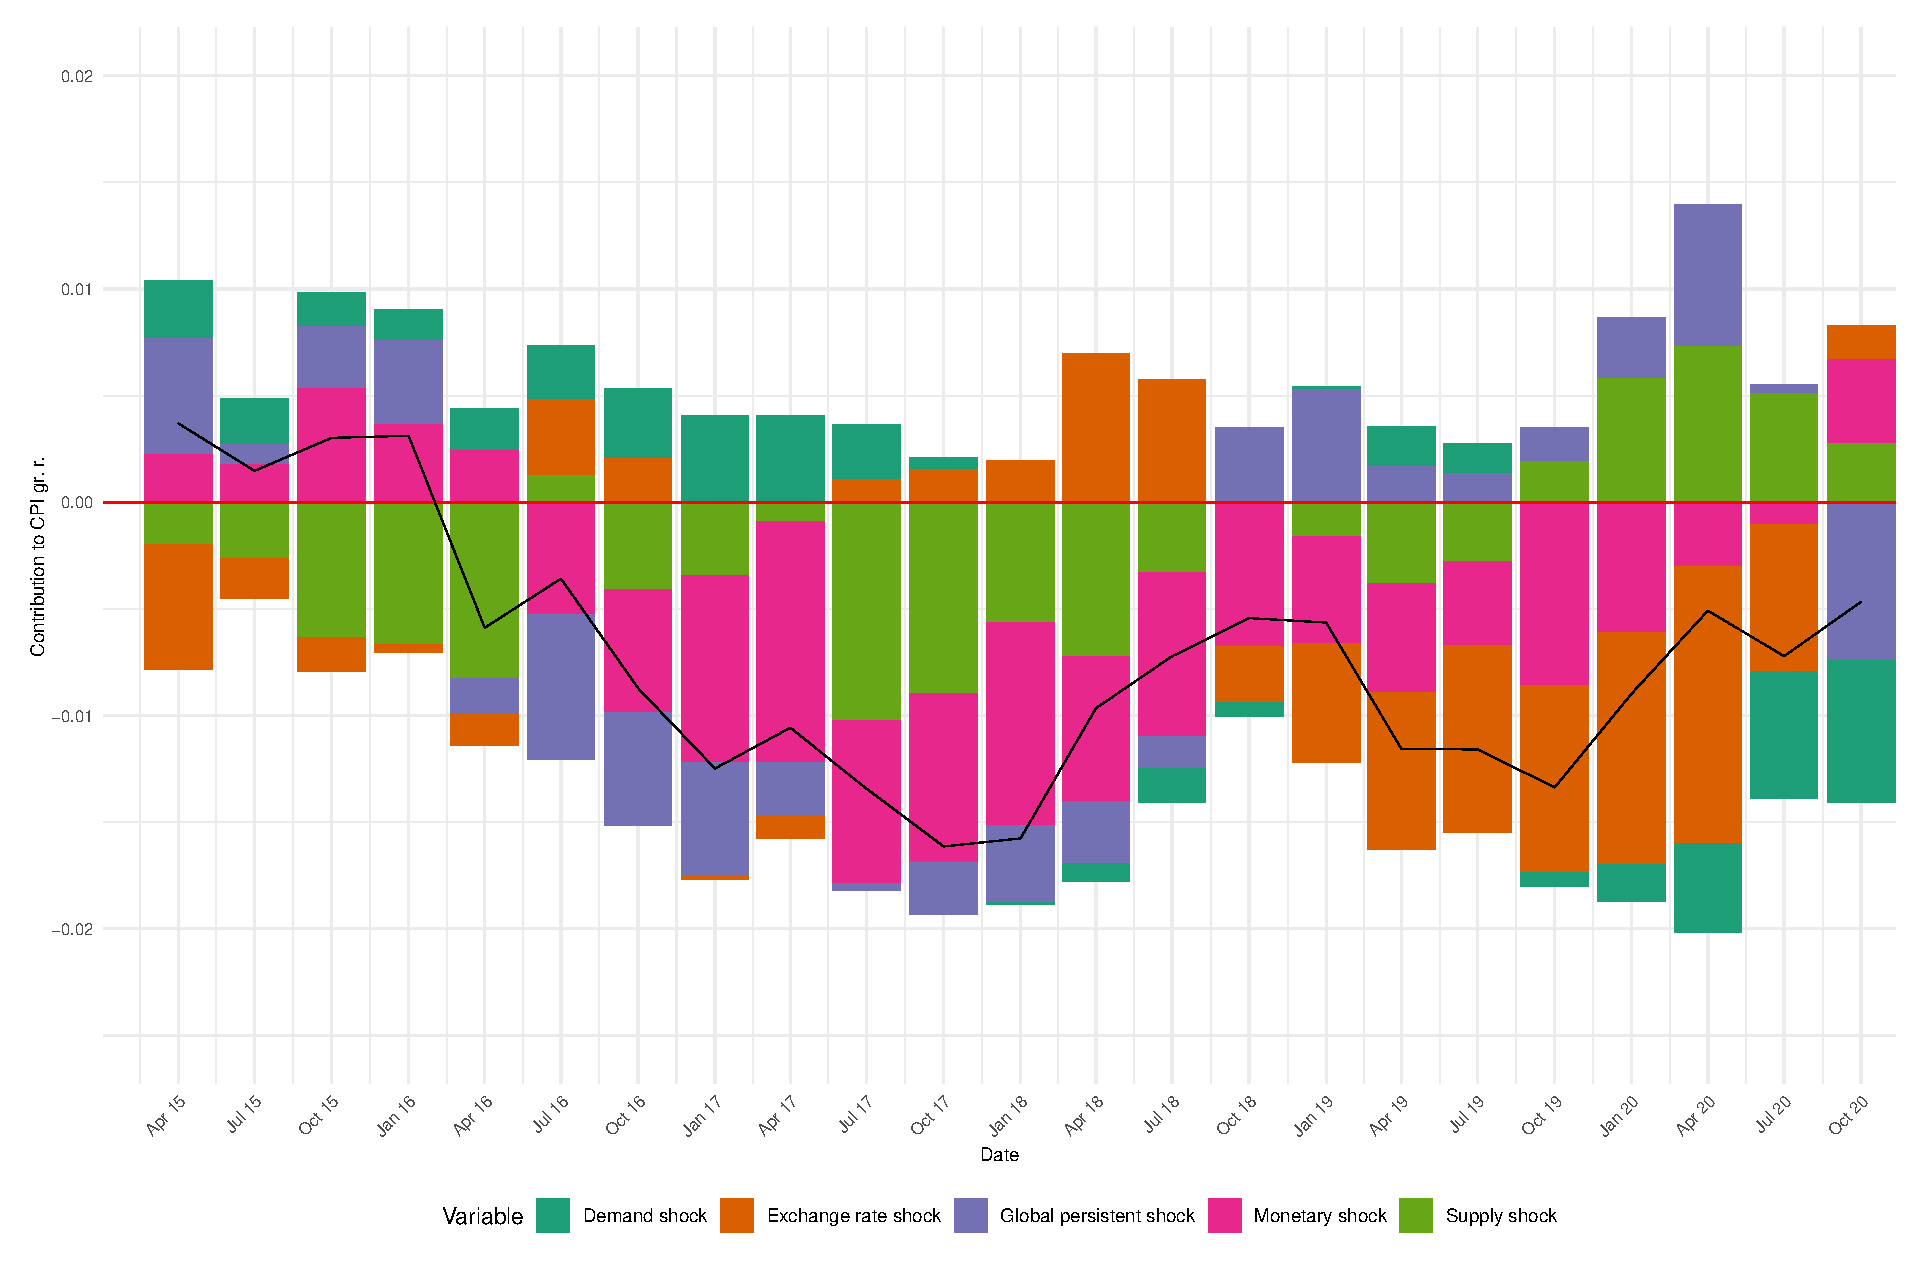
\includegraphics[width=0.95\linewidth]{figures/hd_cpi_cut}
	\caption[]{Historical decomposition of demeaned CPI gr. r. time series (seasonally adjusted), observations from 2015. Black line denotes demeaned observed CPI gr. r.}
	\label{fig:hd_cpi_cut}
\end{sidewaysfigure}

\begin{sidewaysfigure}[h!]
	\centering
	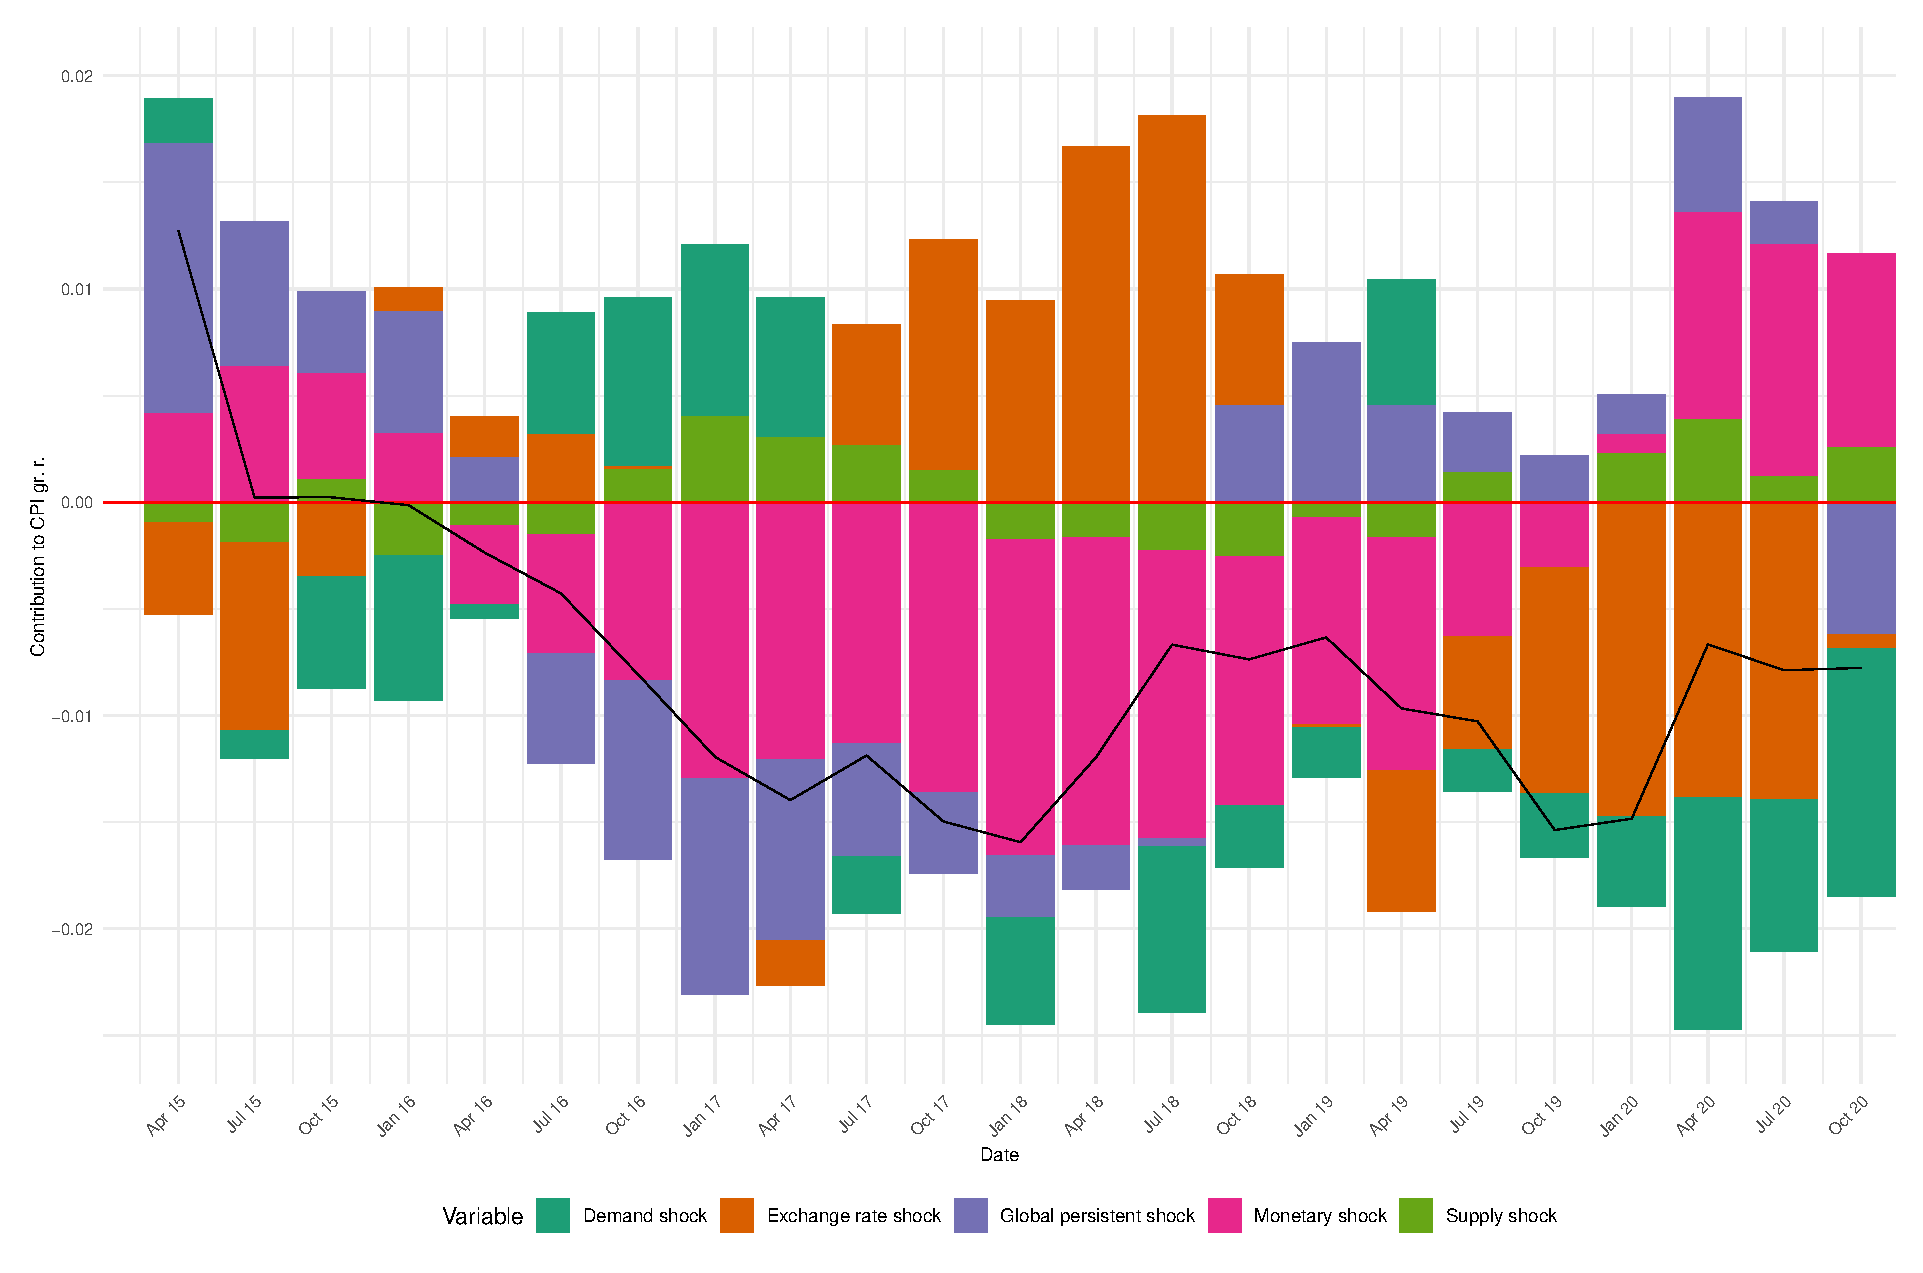
\includegraphics[width=0.95\linewidth]{figures/hd_core_cpi_cut}
	\caption[]{Historical decomposition of demeaned core CPI gr. r. time series (seasonally adjusted), observations from 2015. Black line denotes demeaned observed core CPI gr. r.}
	\label{fig:hd_core_cpi_cut}
\end{sidewaysfigure}

\begin{figure}[h!]
	\centering
	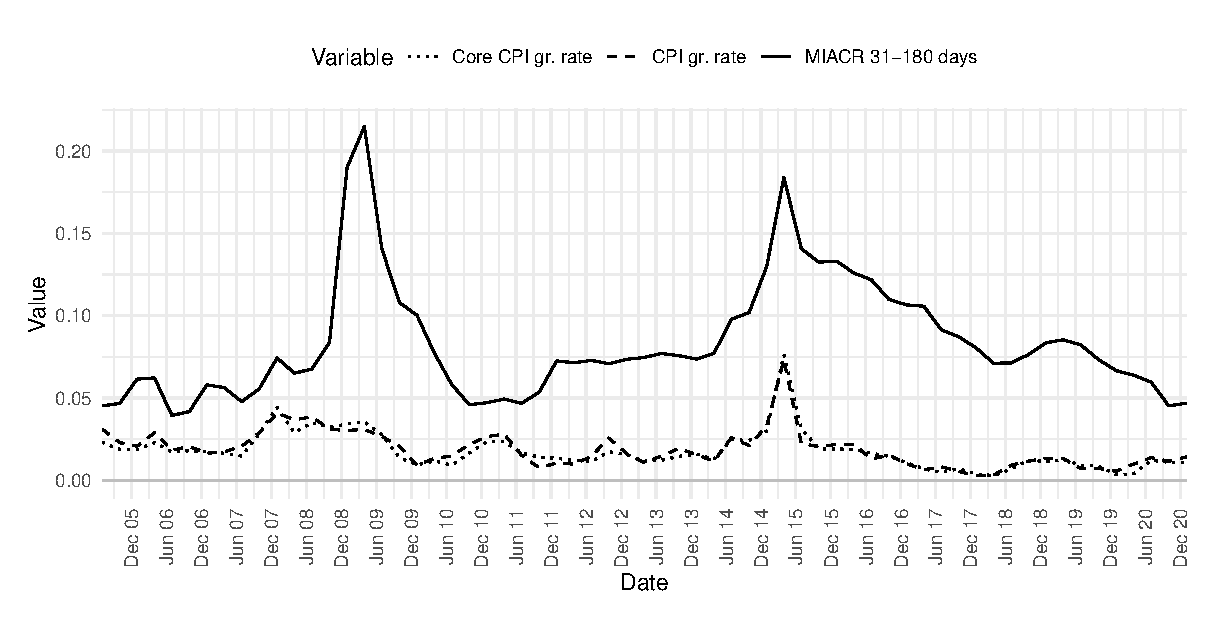
\includegraphics[width=1\linewidth]{figures/intrate_cpi}
	\caption[]{Plot of MIACR (31-180 days) and CPI (full and core compositions) gr. rates.}
	\label{fig:intrate_cpi}
\end{figure}

\clearpage
\section*{SECTION 6. CONCLUSION}
\addcontentsline{toc}{section}{SECTION 6. CONCLUSION}


%%%%%%%%%%%%%%%%%%%%
\renewcommand*{\newblockpunct}{\addperiod\space\bibsentence}
\newpage
\linespread{1.3}

\printbibliography
\addcontentsline{toc}{section}{References}
\newpage
%counters in captions
\setcounter{figure}{0}
\setcounter{table}{0}
\makeatletter
\renewcommand*{\thetable}{\alph{table}}
\renewcommand*{\thefigure}{\alph{figure}}
\let\c@table\c@figure
\makeatother 

%\normalsize
%\linespread{0.5}
\section*{Annex}
\addcontentsline{toc}{section}{Annex}
\label{app}

\begin{table}[h!]
\centering
	%\begin{tabular}{rllllll}
	\begin{tabular}{@{}rlllll@{}}
	  \toprule
	 & Oil price & MIACR & NEER & GDP & CPI \\ 
	  \midrule
	 	Oil price & 1 &  &  &  &\\ 
  		%Import price &  0.12  & 1 &  &  &  &\\ 
  		MIACR& -0.37**  & 1 &  &  & \\ 
  		NEER & -0.45*** & 0.24  &  1  & & \\ 
  		GDP &  0.43***  &  -0.65*** & -0.25* & 1 & \\ 
  		CPI & -0.10  & 0.34  &  0.35** &  -0.08 & 1 \\ 
	   \bottomrule
	\end{tabular}
	\caption{Correlation table (Pearson) of variables, growth rates where applicable.\\ $^*p<0.05,\; ^{**}p<0.01,\;^{***}p<0.001$.}
	\label{table:correlation_variables}
\end{table}

\begin{table}[h!]
	\centering
	%\resizebox{\textwidth}{!}{%
		\begin{tabular}{@{}lll@{}}
			 \toprule
			Variable & ADF & PP \\
			\midrule
			Oil price, gr. r     & {-4.2347, p\textless{}0.01} &{-6.6924, p\textless{}0.01}   \\
			%Import price, gr. r. & {-4.7868, p\textless{}0.01} & {-10.880, p\textless{}0.01}    \\
			MIACR                & {-2.6818, p$\approx$0.30}          & {-2.5258, p$\approx$0.36}          \\
			NEER, gr. r.         & {-3.1391, p$\approx$0.11} & {-8.9038, p\textless{}0.01}   \\
			Real GDP, gr. r  & {-4.9839, p\textless{}0.01} & {-3.9216, p$\approx$0.02} \\
			CPI, gr. r.          & {-3.3366, p$\approx$0.07}         & {-4.4526, p\textless{}0.01}\\
			\bottomrule
		\end{tabular}%
	%}
	\caption{Unit root tests for time series used in the model. Null hypothesis for both models: unit root, alternative hypothesis: stationarity.}
	\label{table:unit_roots}
\end{table}

\begin{sidewaysfigure}[h!]
	\centering
	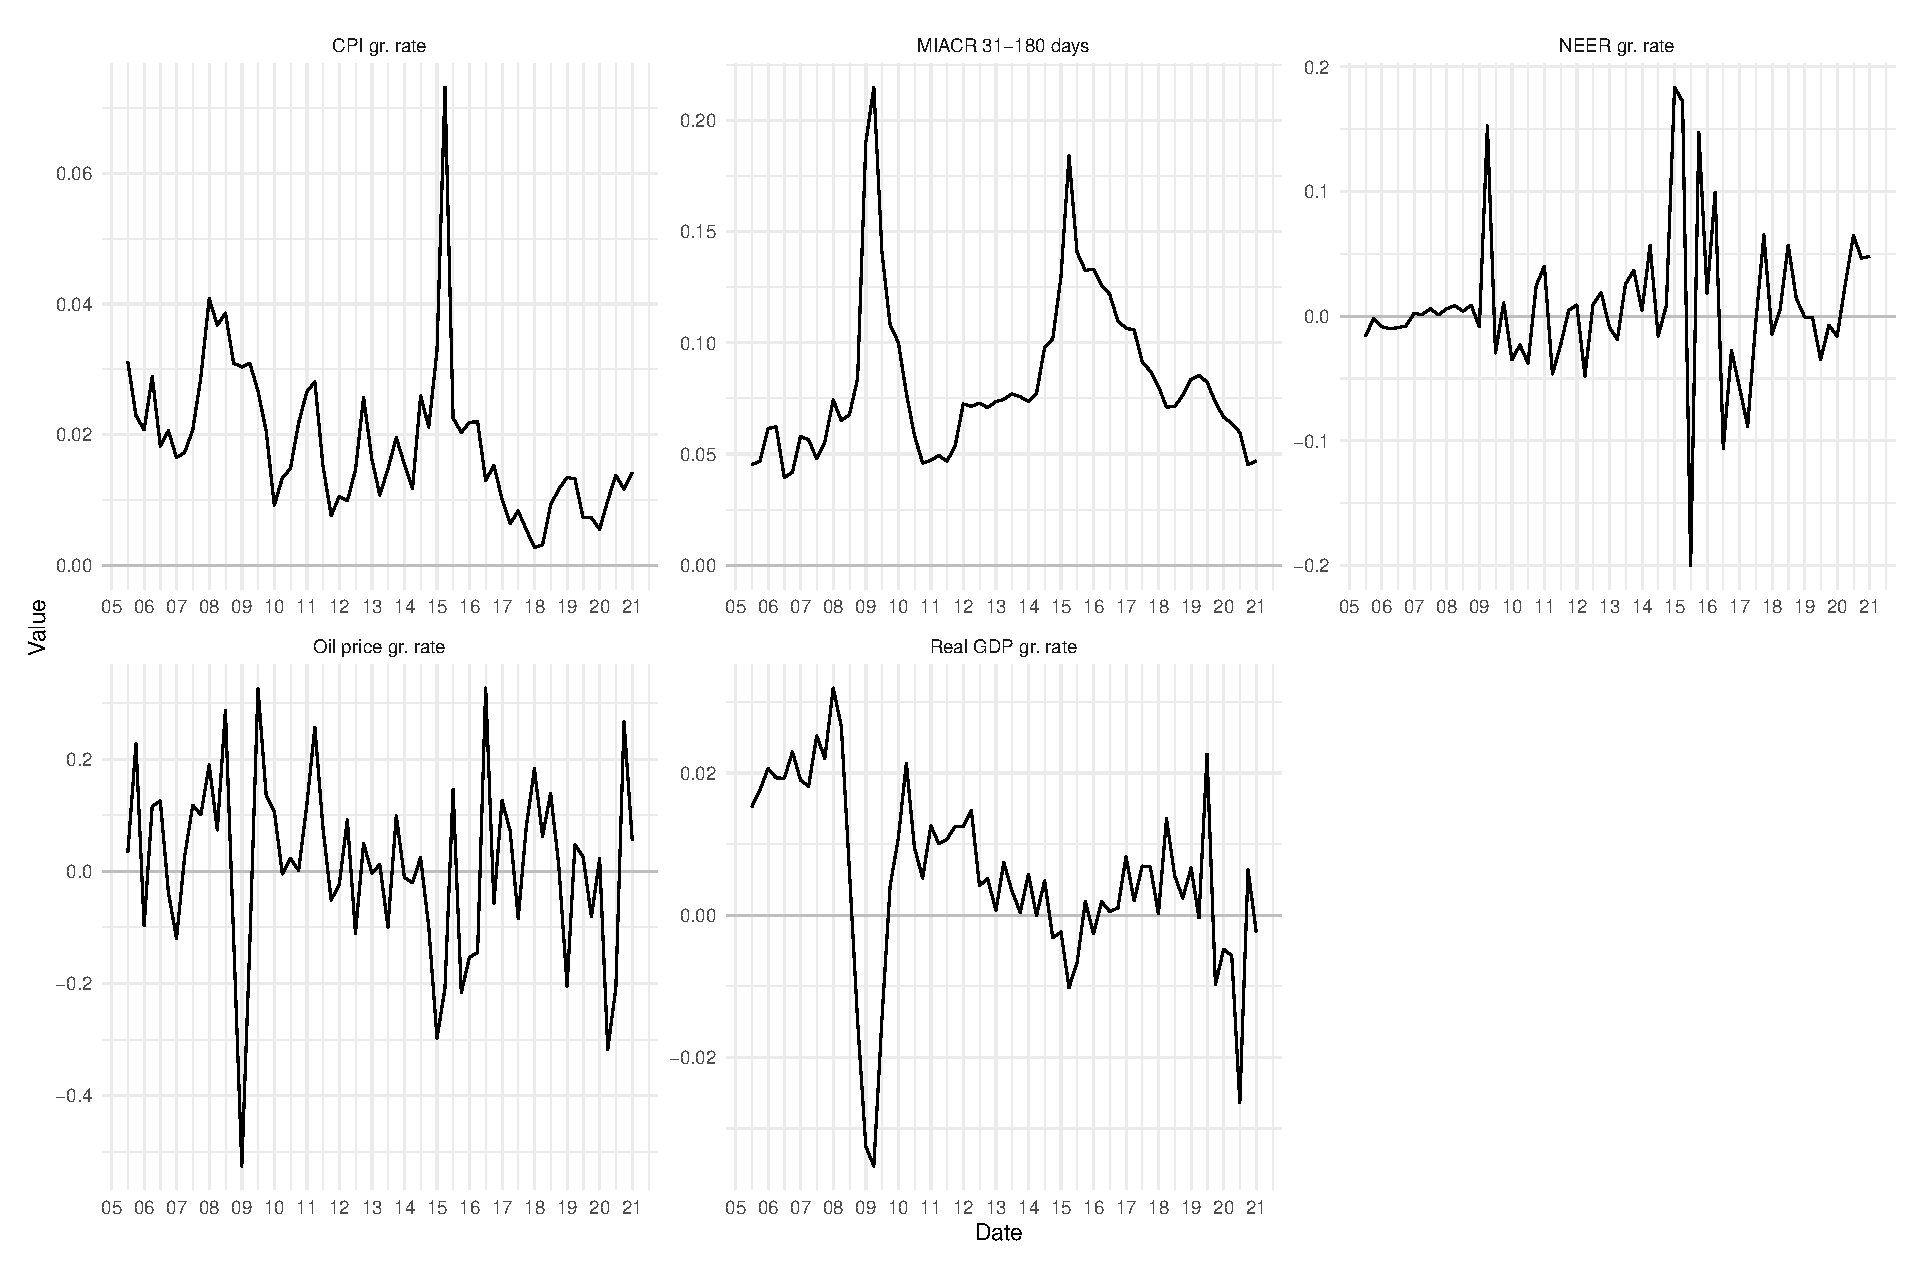
\includegraphics[width=0.9\linewidth]{figures/time_series}
	\caption[]{Time series of variables used in the model, seasonally adjusted. Growth rates, where applicable.}
	\label{fig:timeseries}
\end{sidewaysfigure}

\begin{sidewaysfigure}[h!]
	\centering
	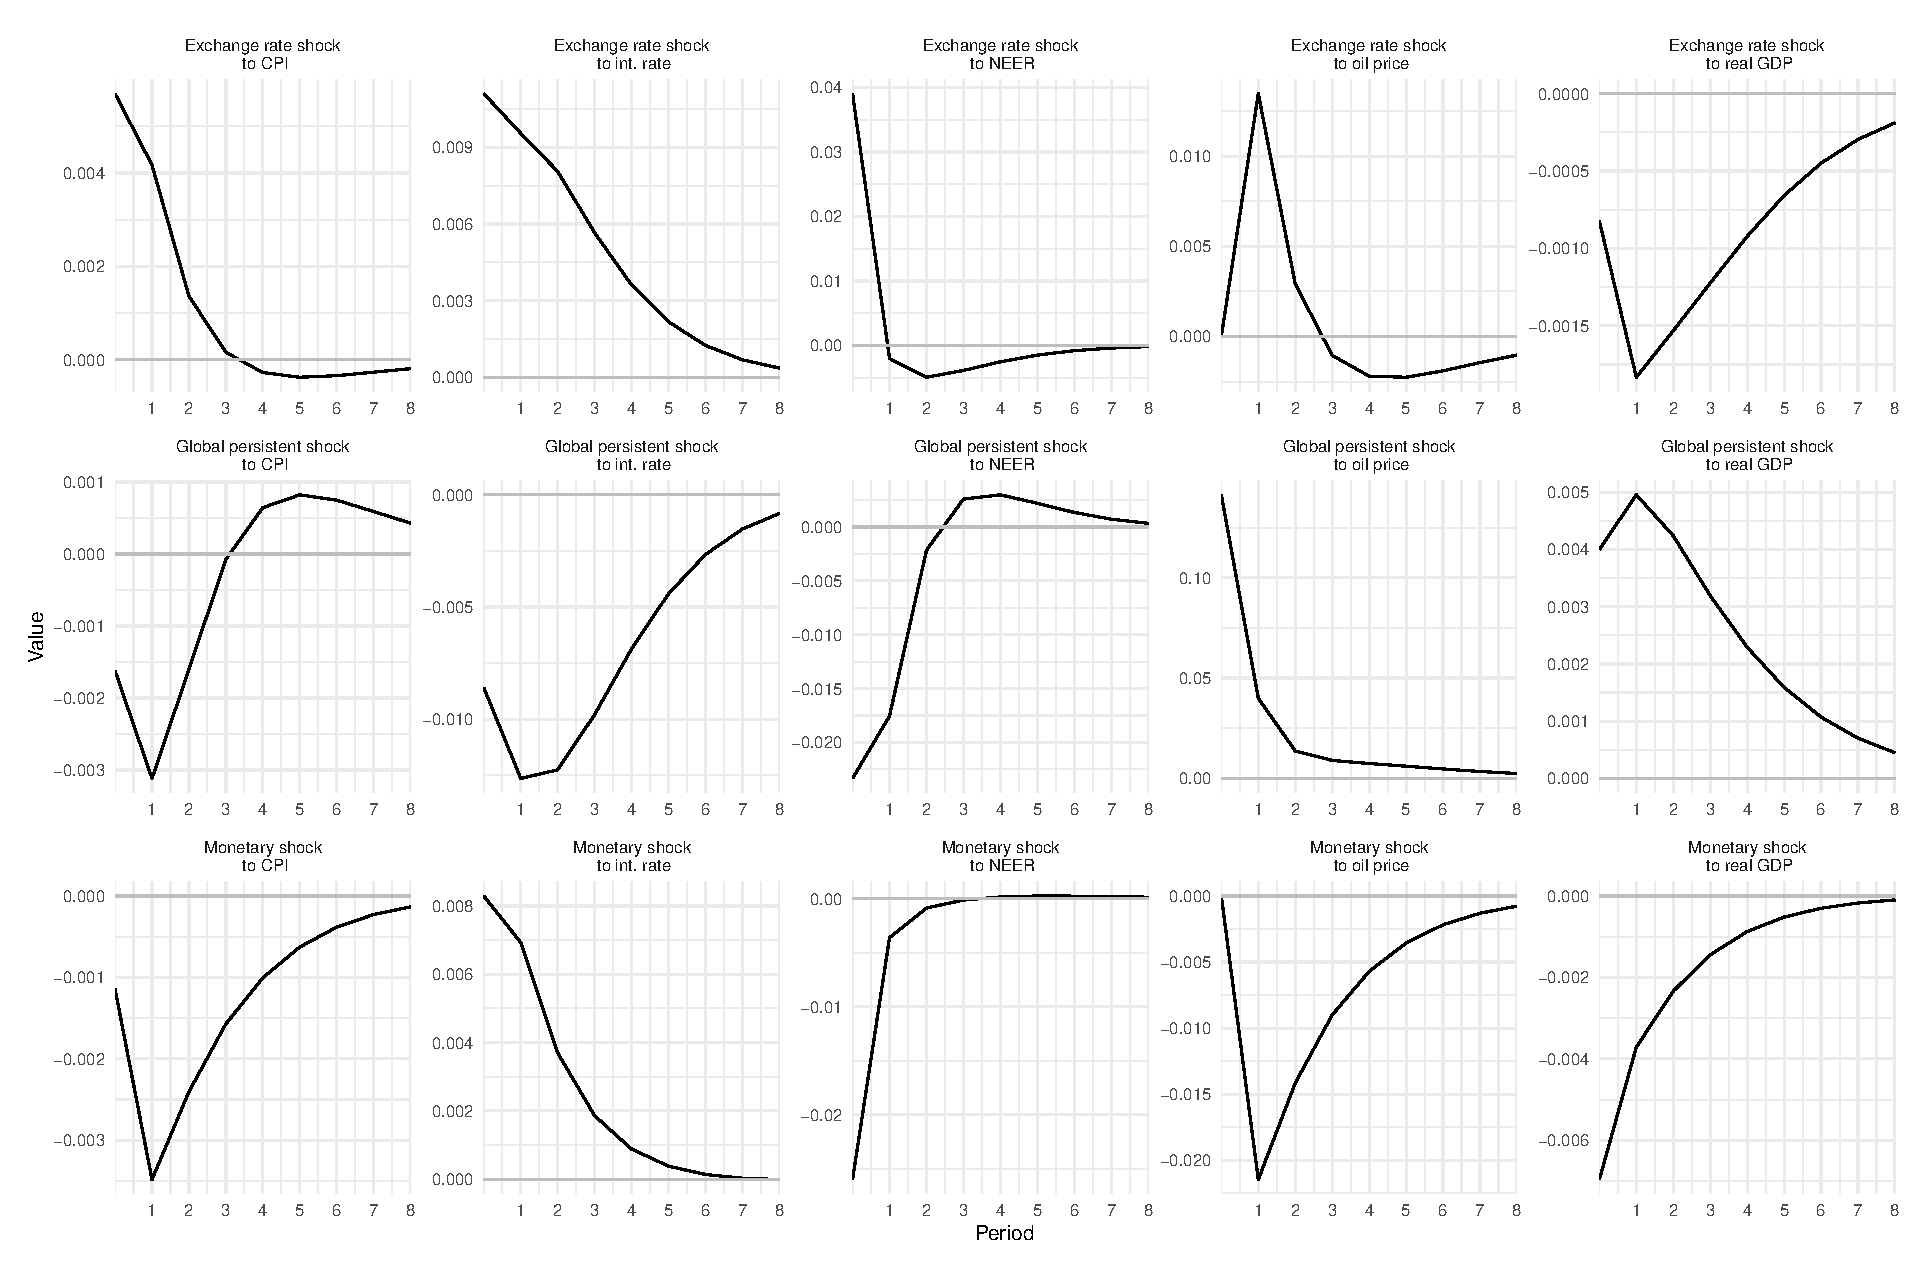
\includegraphics[width=0.9\linewidth]{figures/irf_1}
	\caption[]{Impulse response functions for zero and sign identification scheme, full CPI (1).}
	\label{fig:irf_1}
\end{sidewaysfigure}

\begin{sidewaysfigure}[h!]
	\centering
	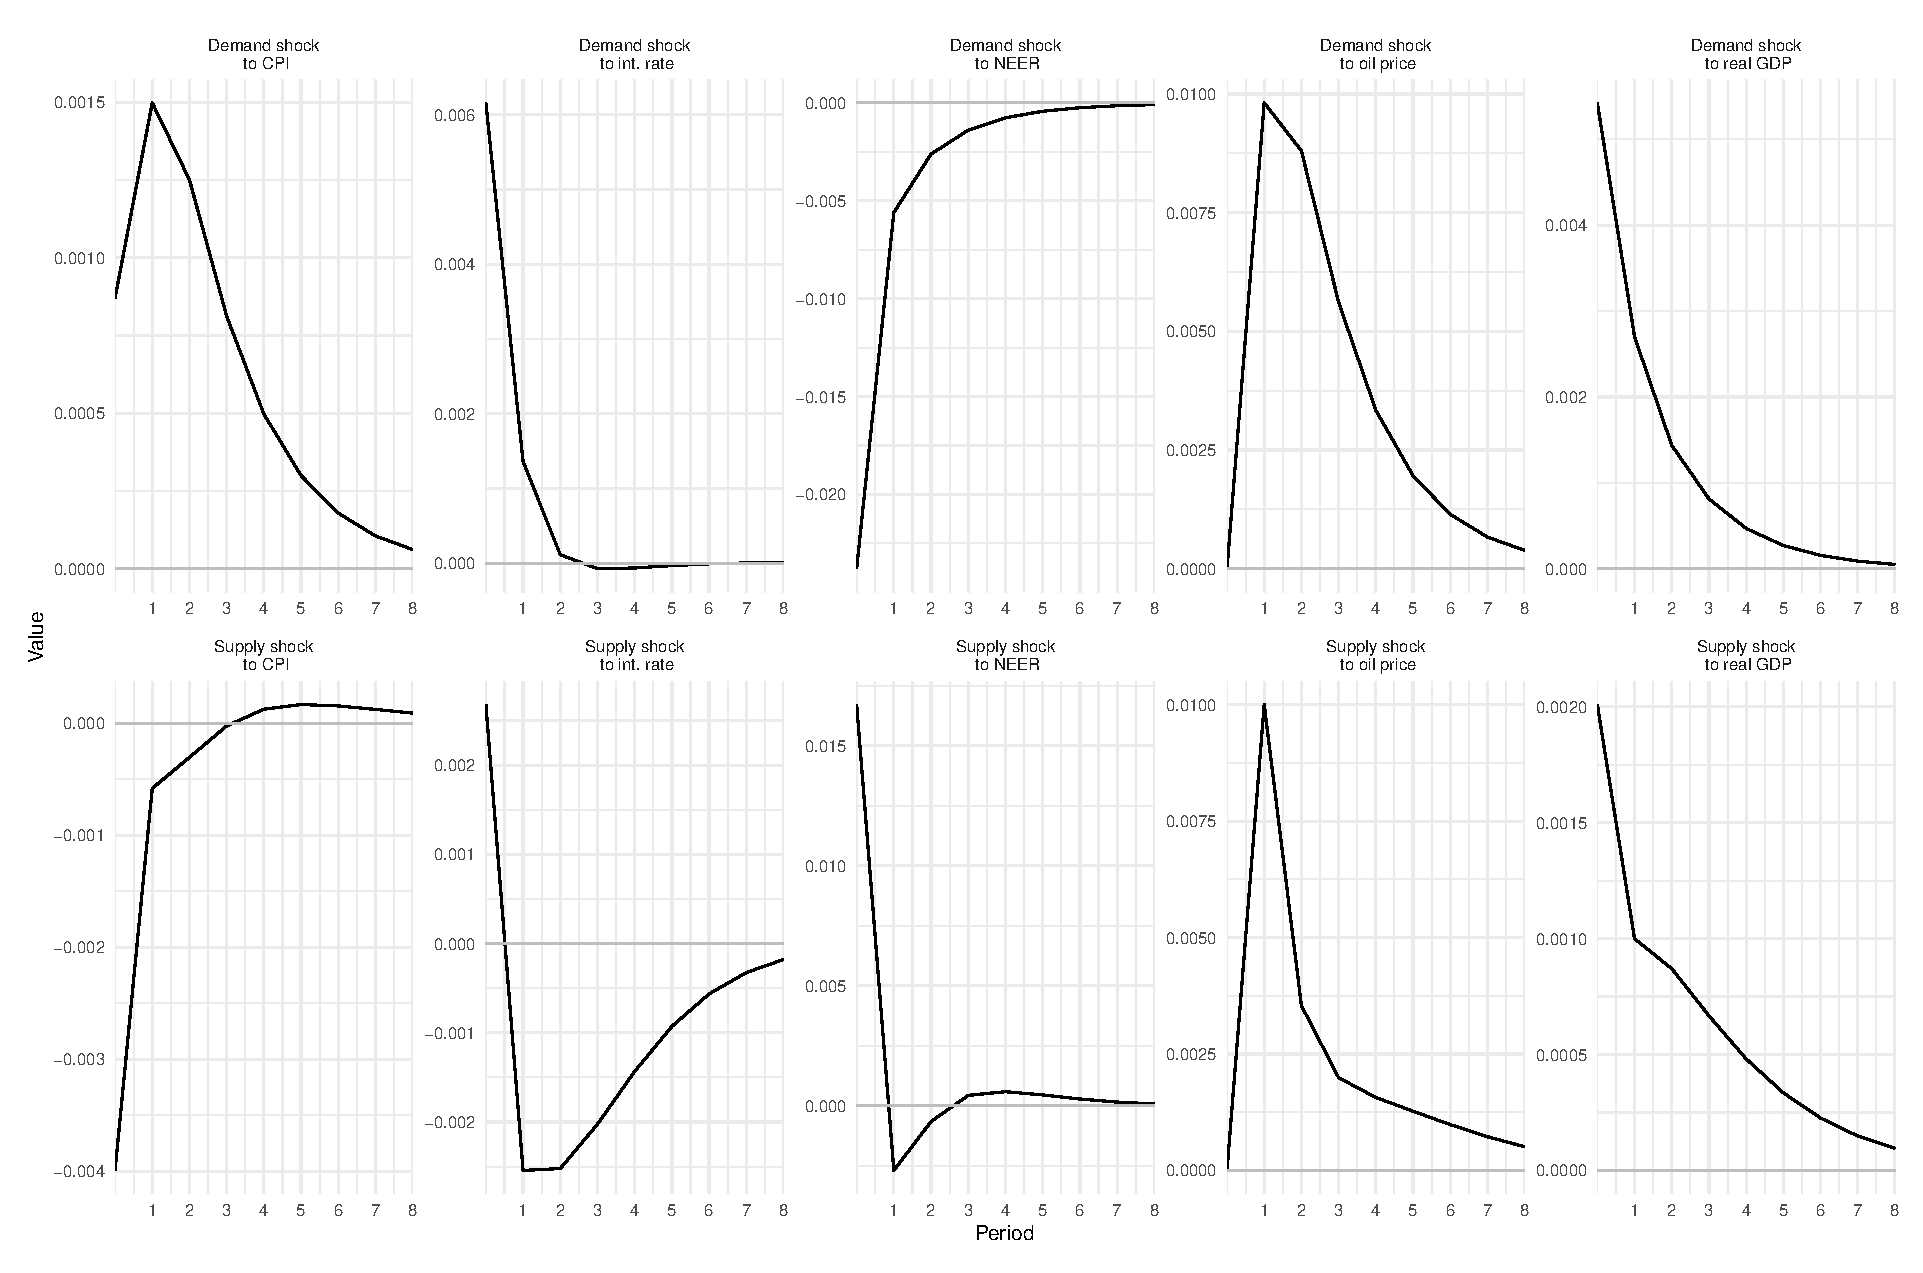
\includegraphics[width=0.9\linewidth]{figures/irf_2}
	\caption[]{Impulse response functions for zero and sign identification scheme, full CPI (2).}
	\label{fig:irf_2}
\end{sidewaysfigure}

\begin{sidewaysfigure}[h!]
	\centering
	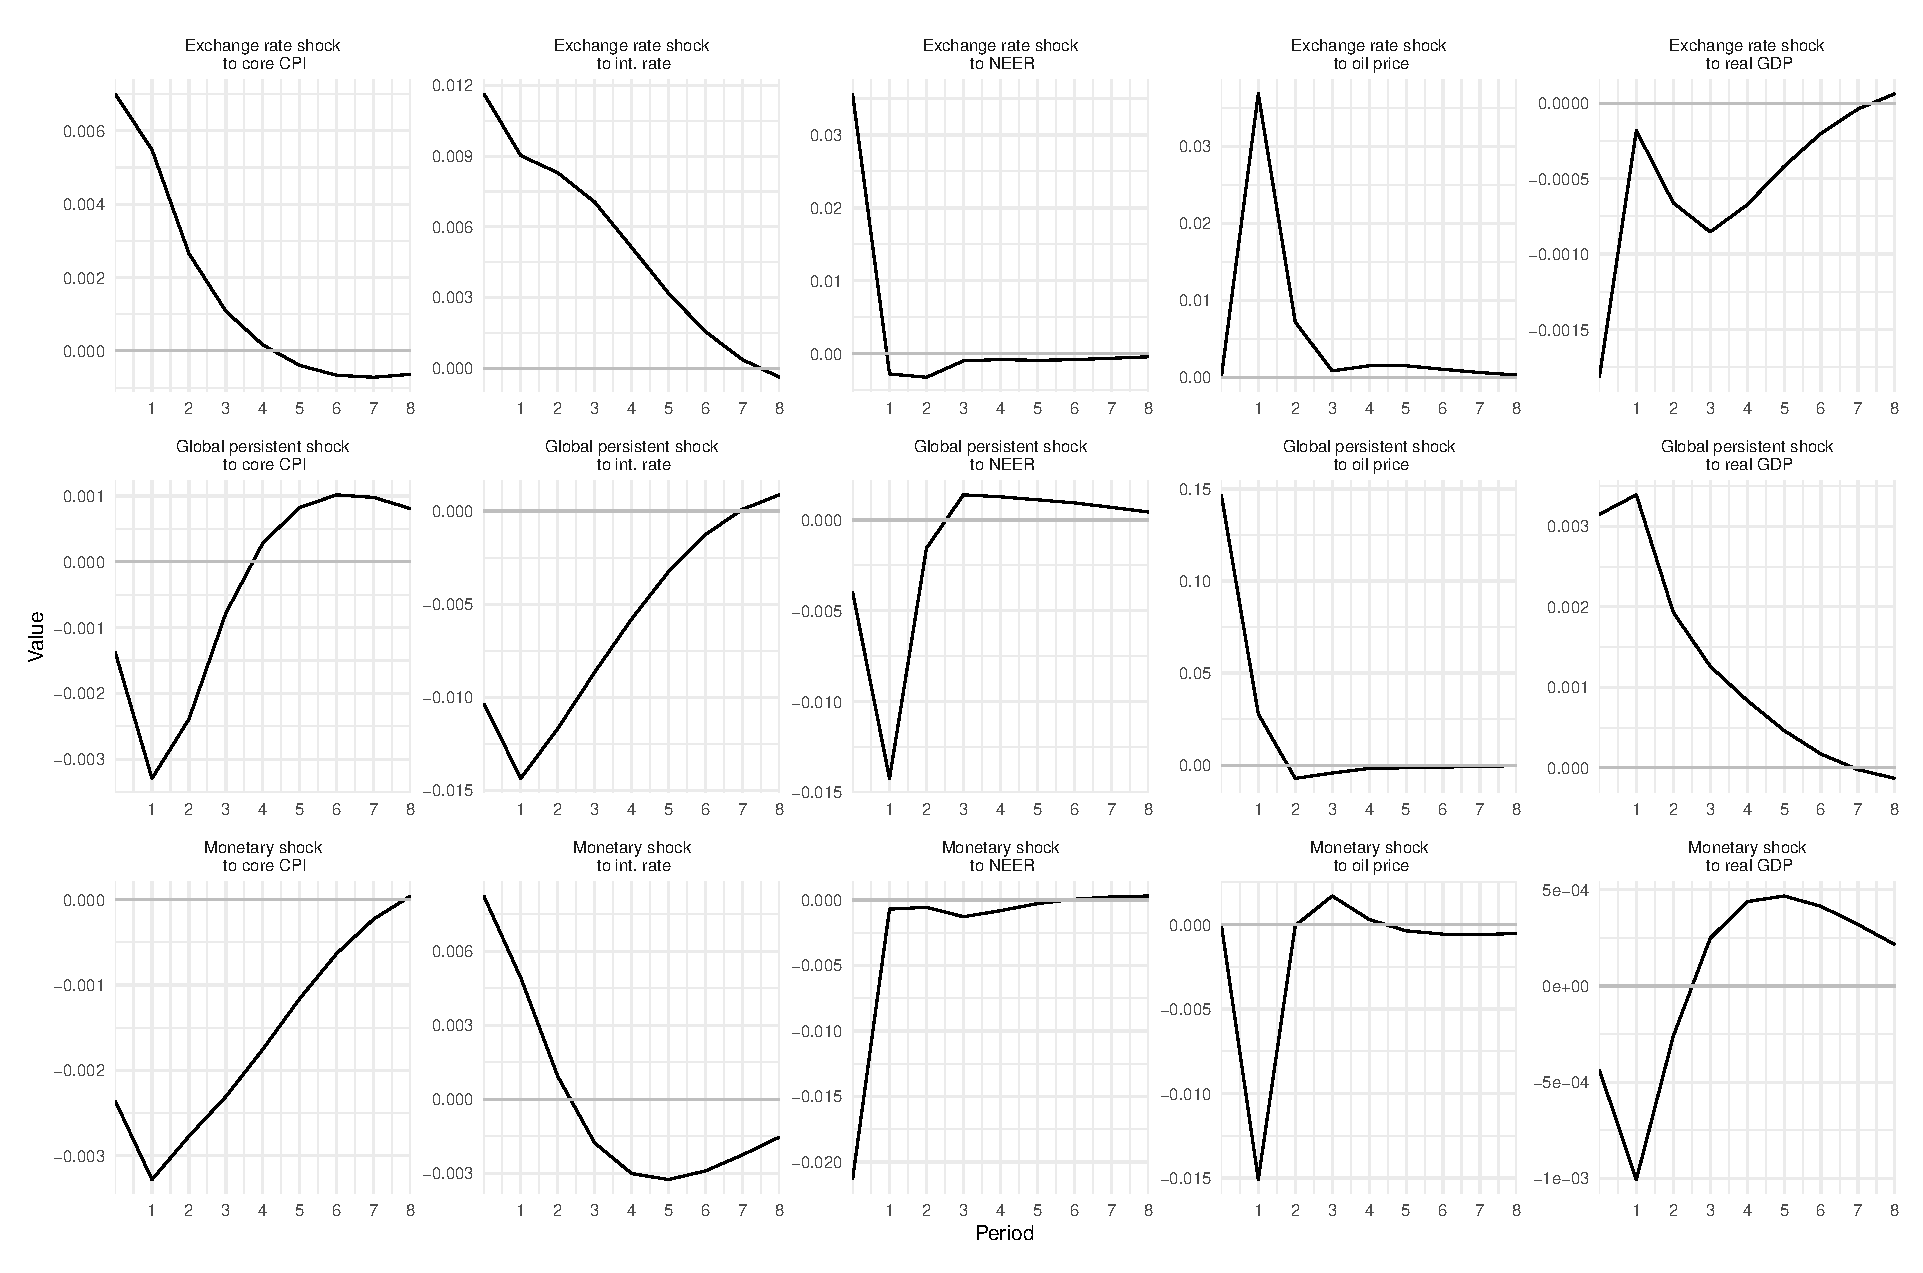
\includegraphics[width=0.9\linewidth]{figures/irf_core_1}
	\caption[]{Impulse response functions for zero and sign identification scheme, core CPI (1).}
	\label{fig:irf_core_1}
\end{sidewaysfigure}

\begin{sidewaysfigure}[h!]
	\centering
	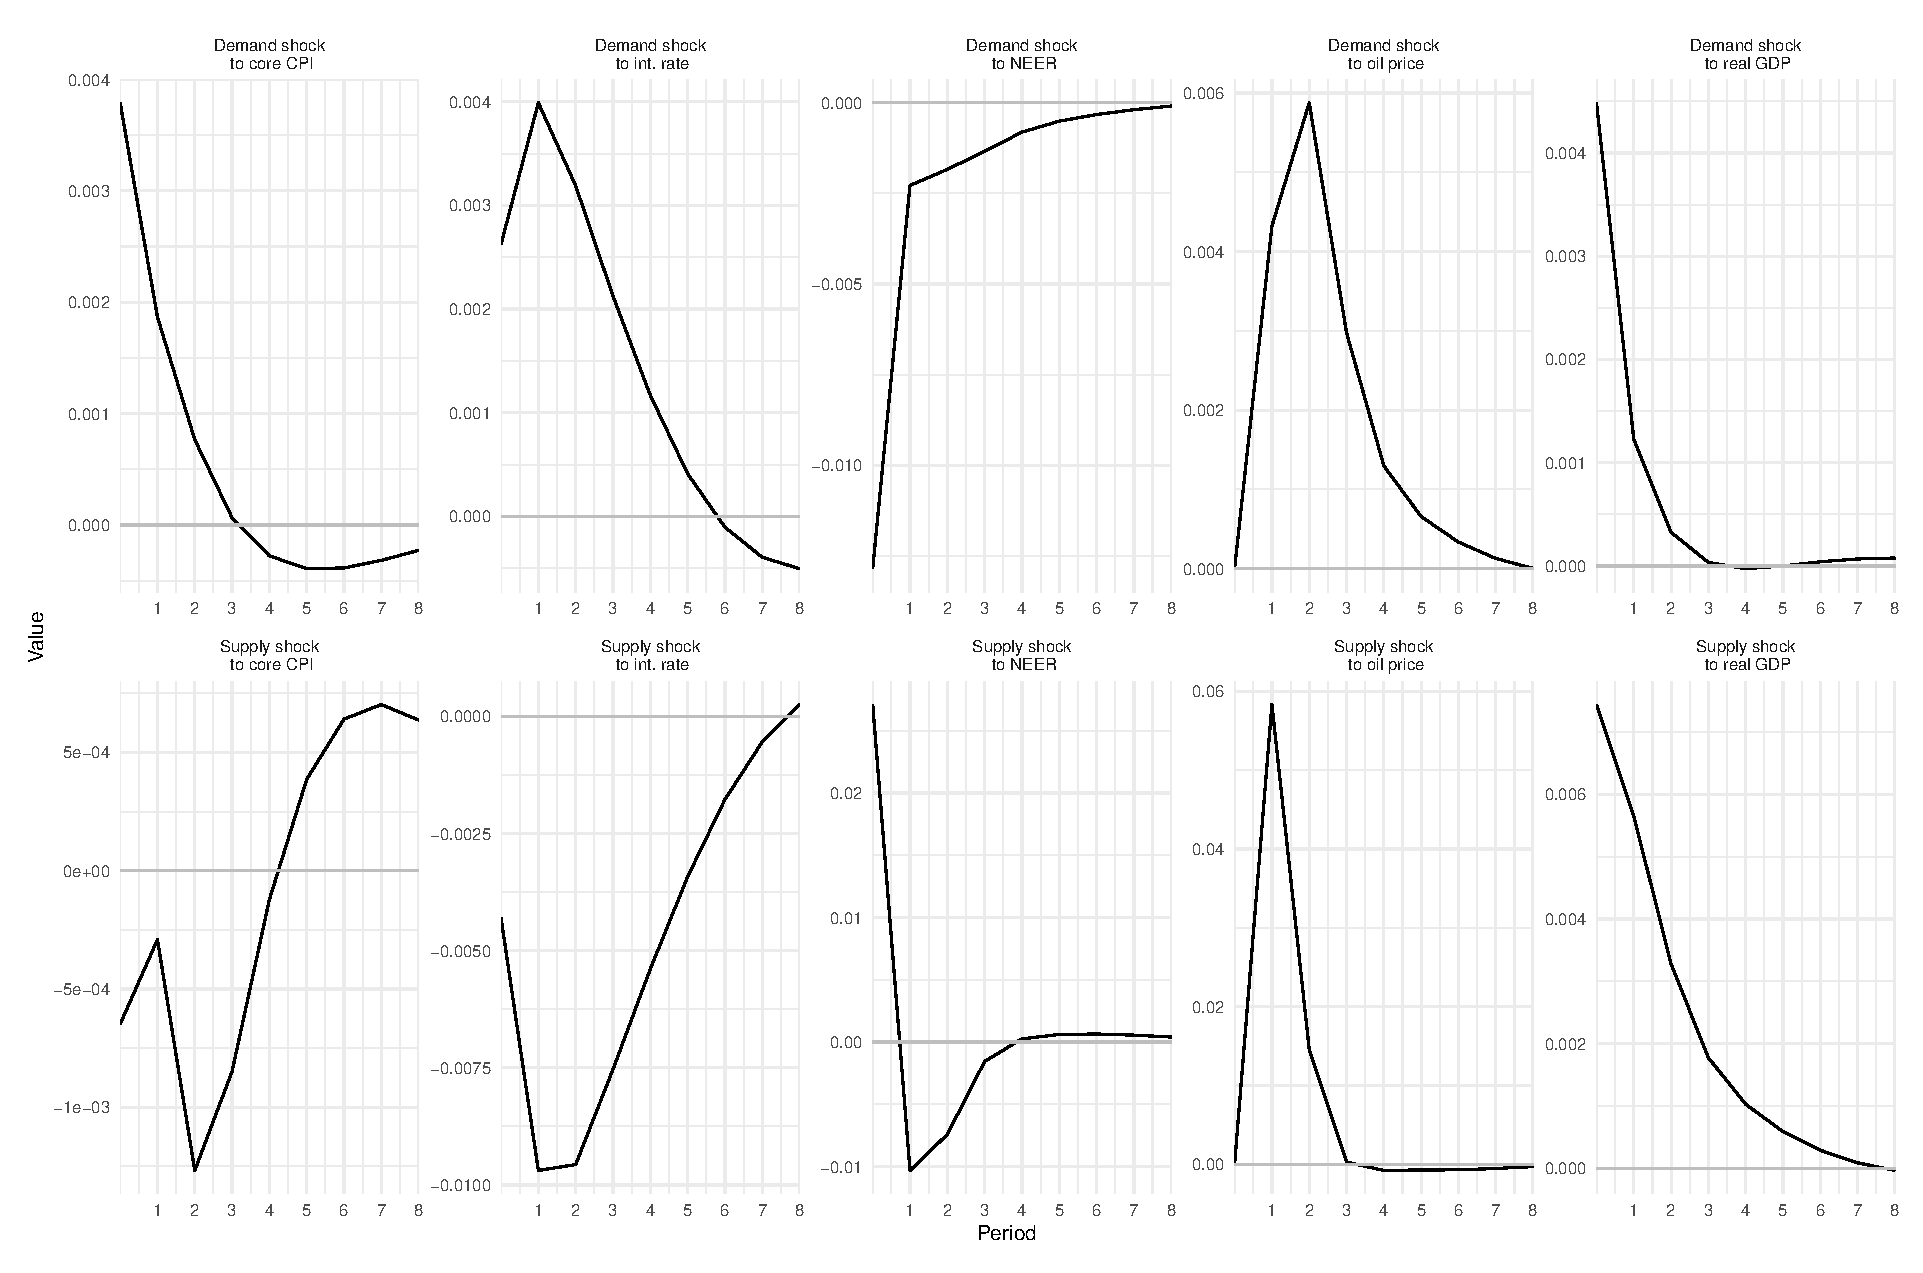
\includegraphics[width=0.9\linewidth]{figures/irf_core_2}
	\caption[]{Impulse response functions for zero and sign identification scheme, core CPI (2).}
	\label{fig:irf_core_2}
\end{sidewaysfigure}

\begin{sidewaysfigure}[h!]
	\centering
	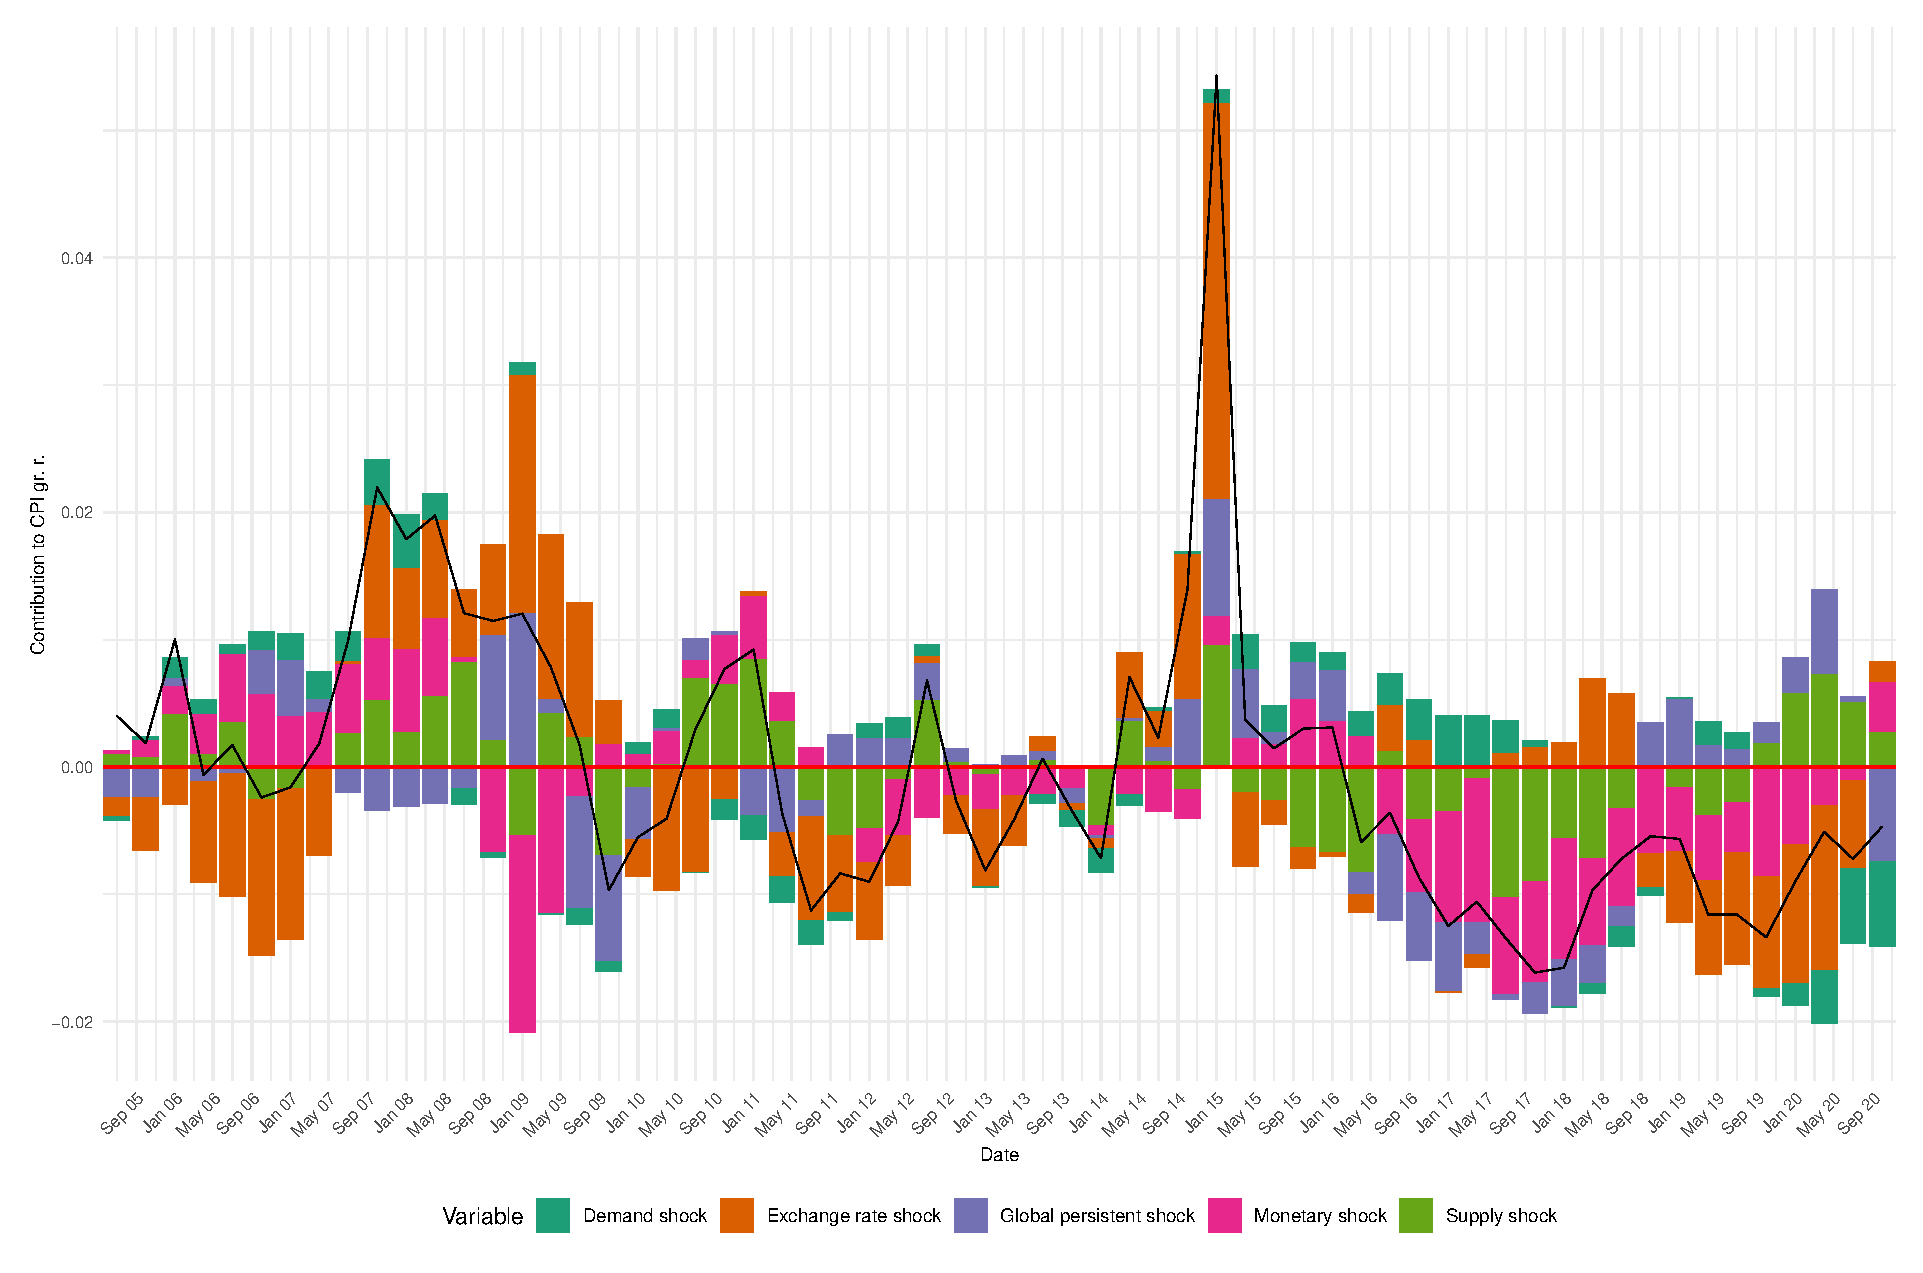
\includegraphics[width=0.95\linewidth]{figures/hd_cpi_full}
	\caption[]{Historical decomposition of demeaned CPI gr. r. time series (seasonally adjusted). Black line denotes demeaned observed CPI gr. r.}
	\label{fig:hd_cpi_full}
\end{sidewaysfigure}

\begin{sidewaysfigure}[h!]
	\centering
	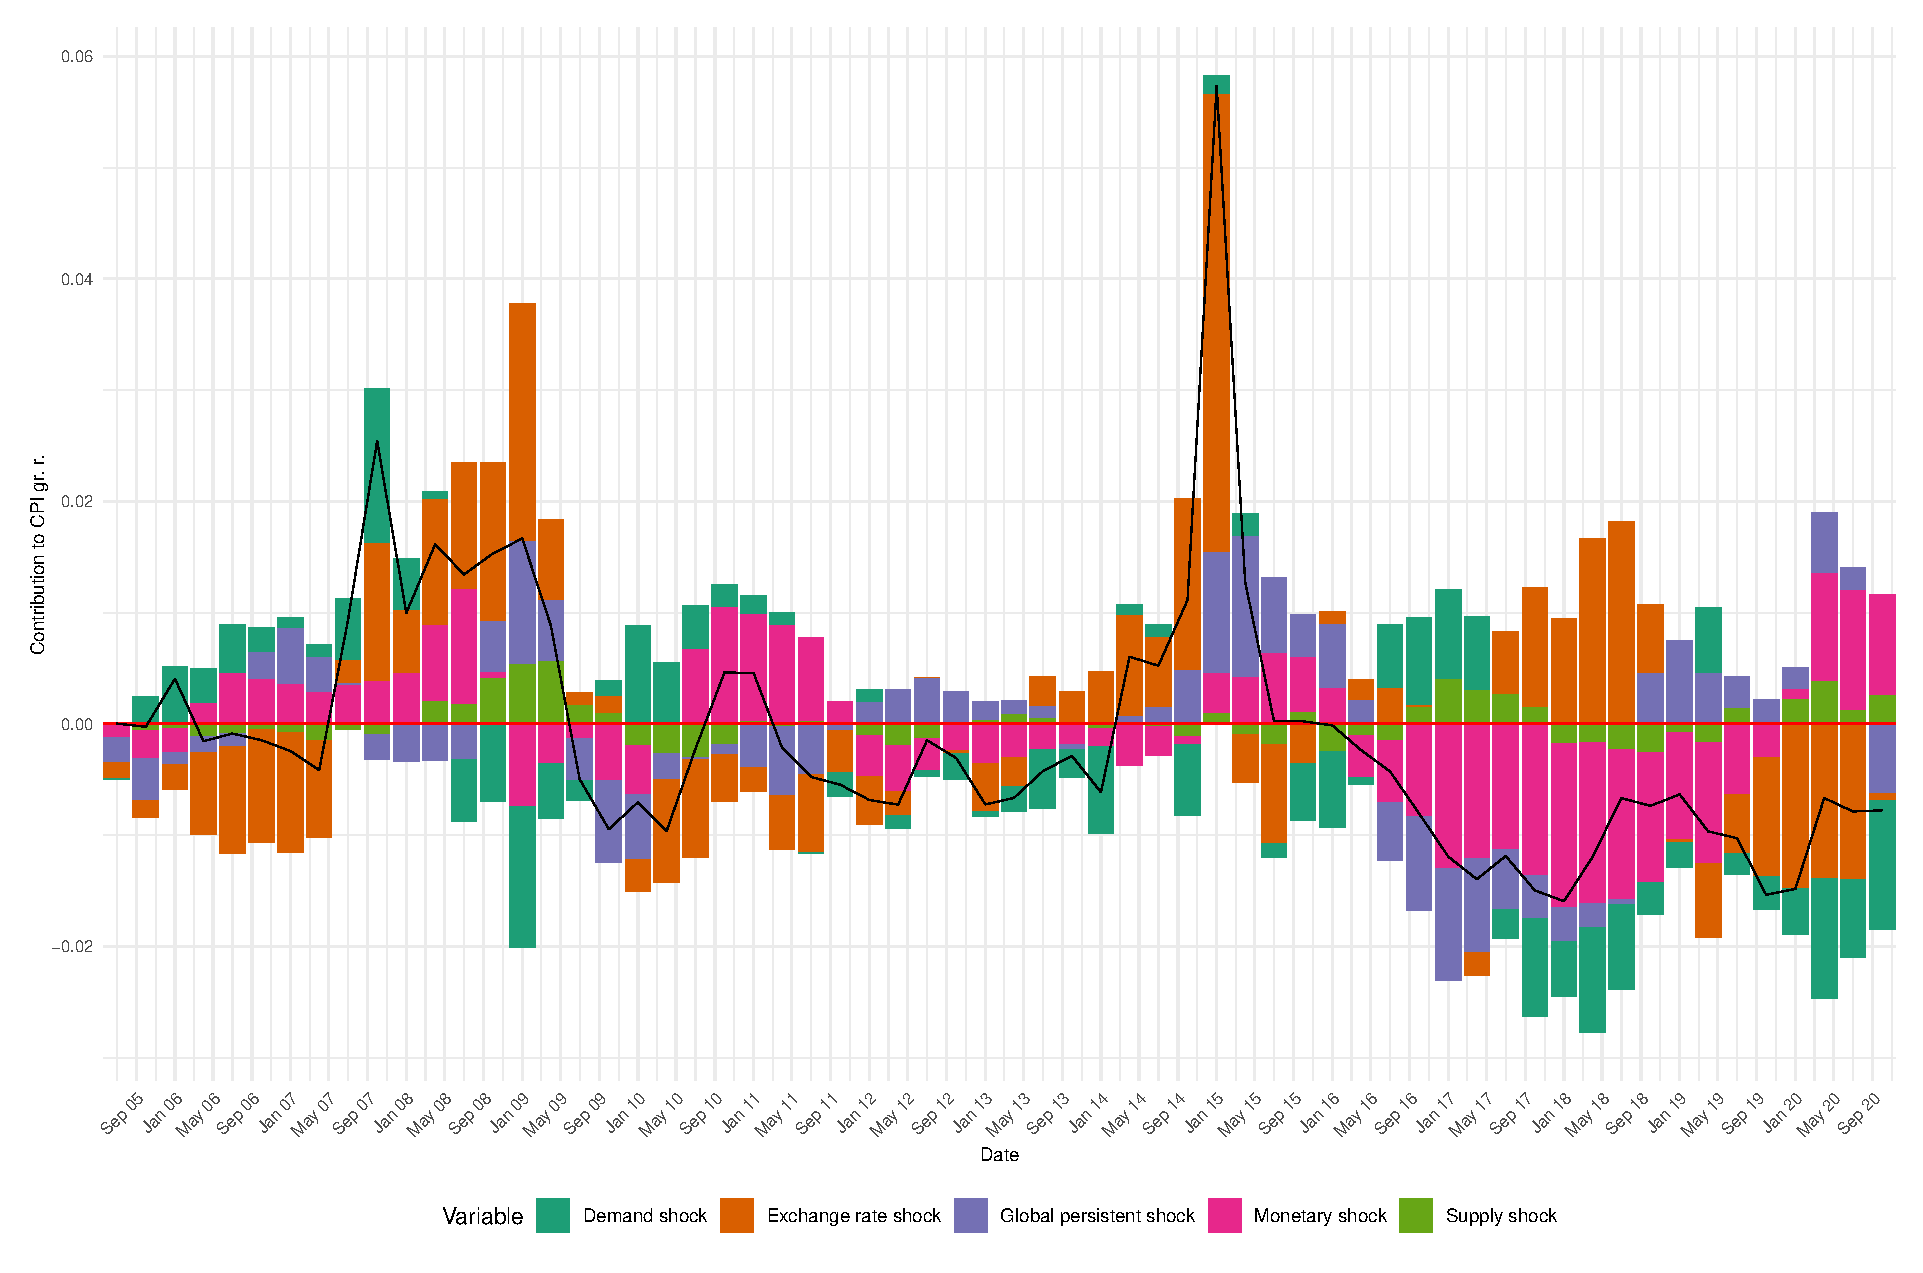
\includegraphics[width=0.95\linewidth]{figures/hd_core_cpi_full}
	\caption[]{Historical decomposition of demeaned core CPI gr. r. time series (seasonally adjusted). Black line denotes demeaned observed core CPI gr. r.}
	\label{fig:hd_core_cpi_full}
\end{sidewaysfigure}


~\\
\clearpage
\newpage
\pagebreak

\end{document}
